\begin{frame}
    \titlepage
\end{frame}

\setcounter{tocdepth}{1} % Tiefe von Inhaltsverzeichnis
\begin{frame}
    \tableofcontents
\end{frame}

\section{Aufgabenstellung und Produktanforderungen} % Peter
\subsection{Aufgabenstellung}
\section{Aufgabenstellung und Produktanforderungen} % Peter
\subsection{Aufgabenstellung}
\begin{frame}
    \frametitle{Aufgabenstellung}
	\begin{block}{Aufgabenstellung}
	    \begin{itemize}
	    	\item 5 Tennisbälle
	    	\item 1 Korb
		    \item 1 Spielfeld
		    \item 1 Ziel!
	    \end{itemize}
    \end{block}
\end{frame}

\section{Realisierung}
%\begin{frame}
%    \frametitle{Übersicht}
%    \begin{columns}
%        \begin{column}{0.50\textwidth}
%            \centering
%            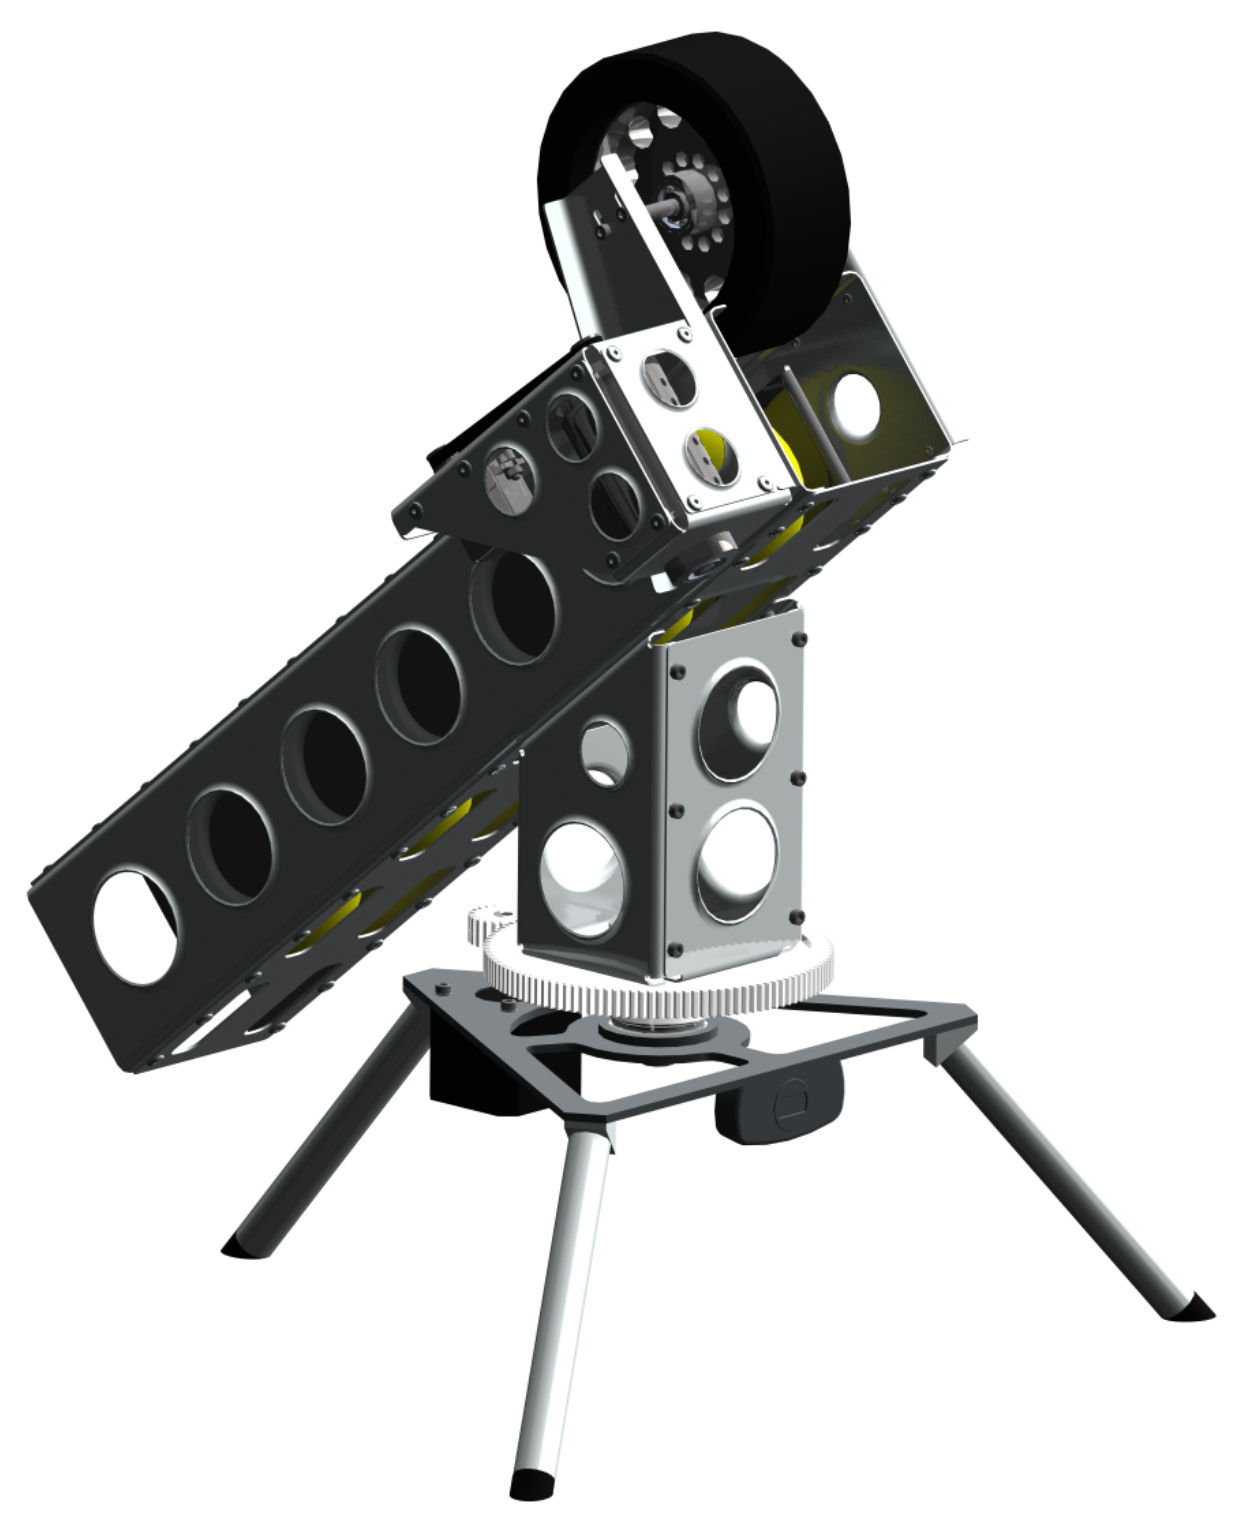
\includegraphics[width=1.00\textwidth]{../doc/fig/Bild_mit_Kamera.png}
%        \end{column}
%        \begin{column}{0.50\textwidth}
%            \begin{block}{Komponenten}
%                \begin{itemize}
%                    \item Kamera
%                    \item Drehvorrichtung
%                    \item Turm
%                    \item Balllager
%                    \item Ballnachschub
%                    \item BLDC Motor
%                \end{itemize}
%            \end{block}
%        \end{column}
%    \end{columns}
%\end{frame}
\begin{frame}
    \frametitle{Übersicht}
    \begin{columns}
        \begin{column}{1.00\textwidth}
            \begin{figure}[h]
                \centering
                \begin{tikzpicture}[scale=1.00]
                    \node[above right] (img) at (0,0) {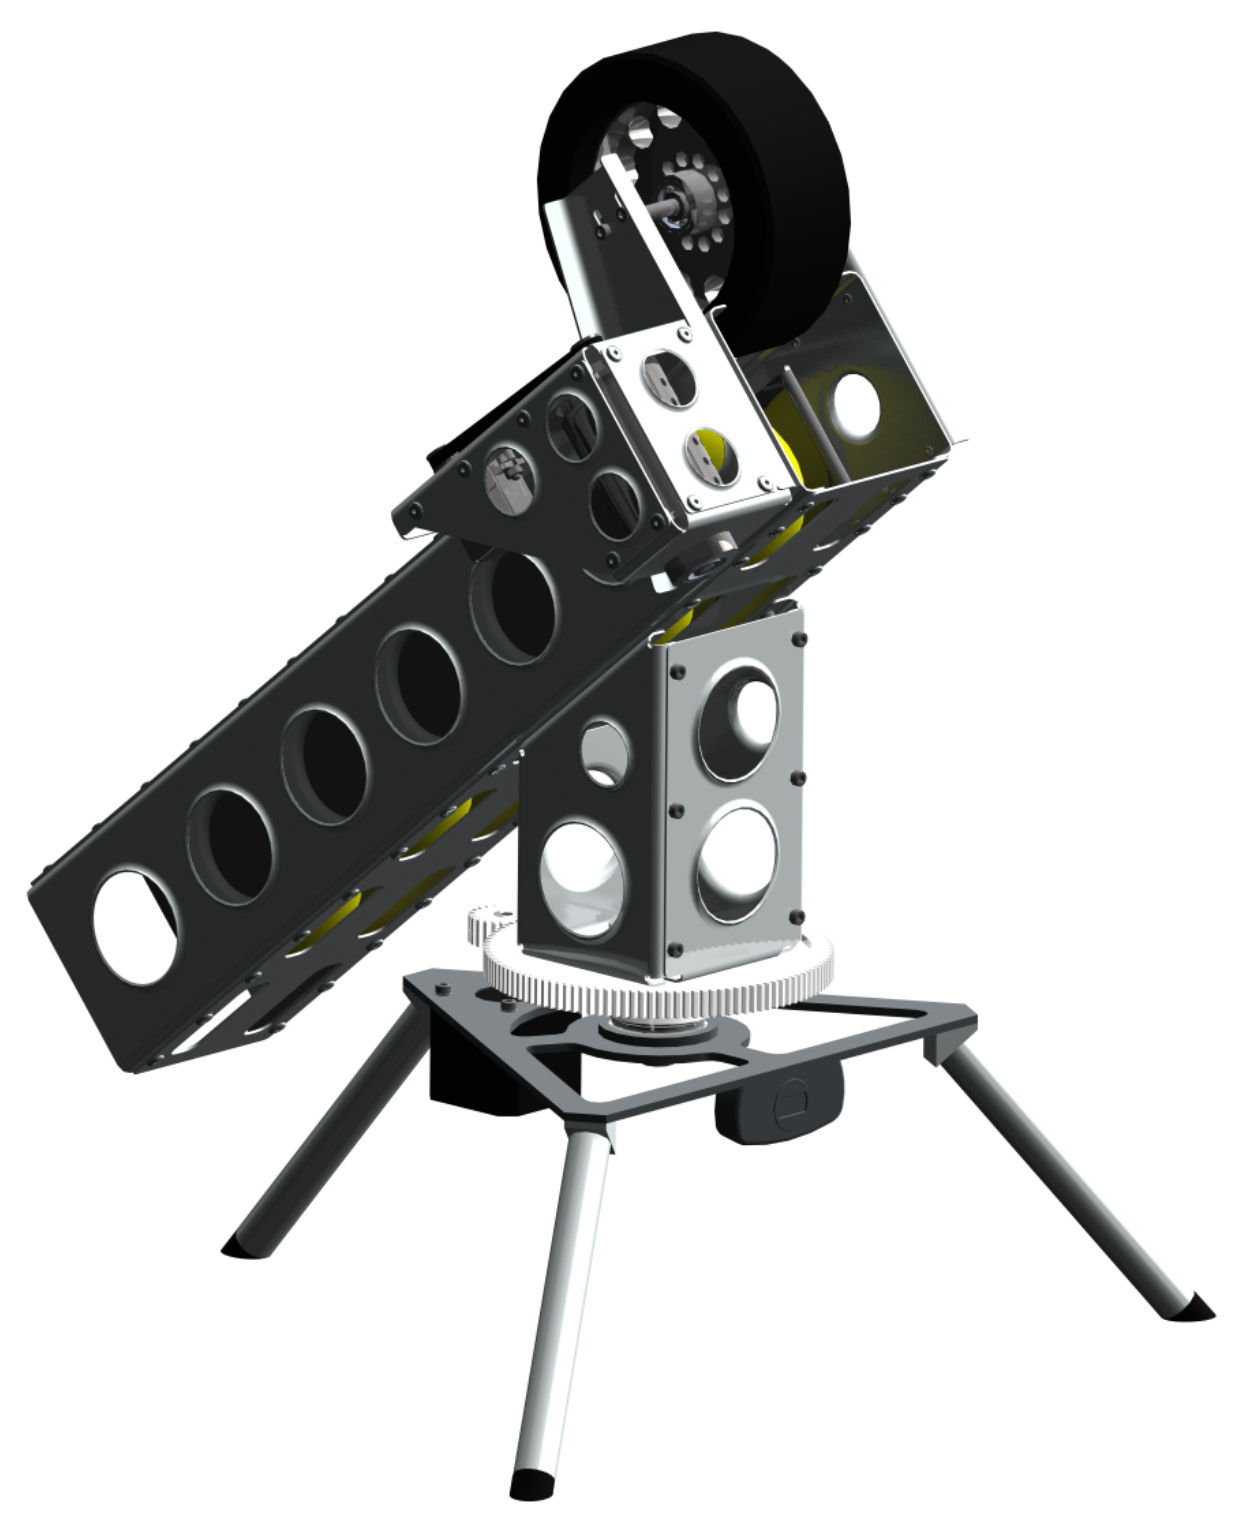
\includegraphics[width=0.50\textwidth]{../doc/fig/Bild_mit_Kamera.png}};
                    \draw[line width=1pt]
                        (0, 4) node[left=0mm] {Balllager}
                        -- (1.5, 3.7);
                    \fill (1.5, 3.7) circle (2pt);
                    \draw[line width=1pt]
                        (1, 5) node[left=0mm] {Ballnachschub}
                        -- (2.5, 4.7);
                    \fill (2.5, 4.7) circle (2pt);
                    \draw[line width=1pt]
                        (6.0, 3.0) node[right=0mm] {Drehvorrichtung}
                        -- (3.0, 2.4);
                    \fill (3.0, 2.4) circle (2pt);
                    \draw[line width=1pt]
                        (5.0, 6.0) node[right=0mm] {BLDC Motor}
                        -- (3.2, 6.0);
                    \fill (3.2, 6.0) circle (2pt);
                    \draw[line width=1pt]
                        (5.5, 4.5) node[right=0mm] {Turm}
                        -- (3.5, 3.5);
                    \fill (3.5, 3.5) circle (2pt);
                    \draw[line width=1pt]
                        (6.5, 1.5) node[right=0mm] {Kamera}
                        -- (3.7, 2.0);
                    \fill (3.7, 2.0) circle (2pt);
                \end{tikzpicture}
            \end{figure}
        \end{column}
    \end{columns}
\end{frame}


\begin{frame}
    \frametitle{Konstruktion}
    \begin{columns}
        \begin{column}{1\textwidth}
            \centering
            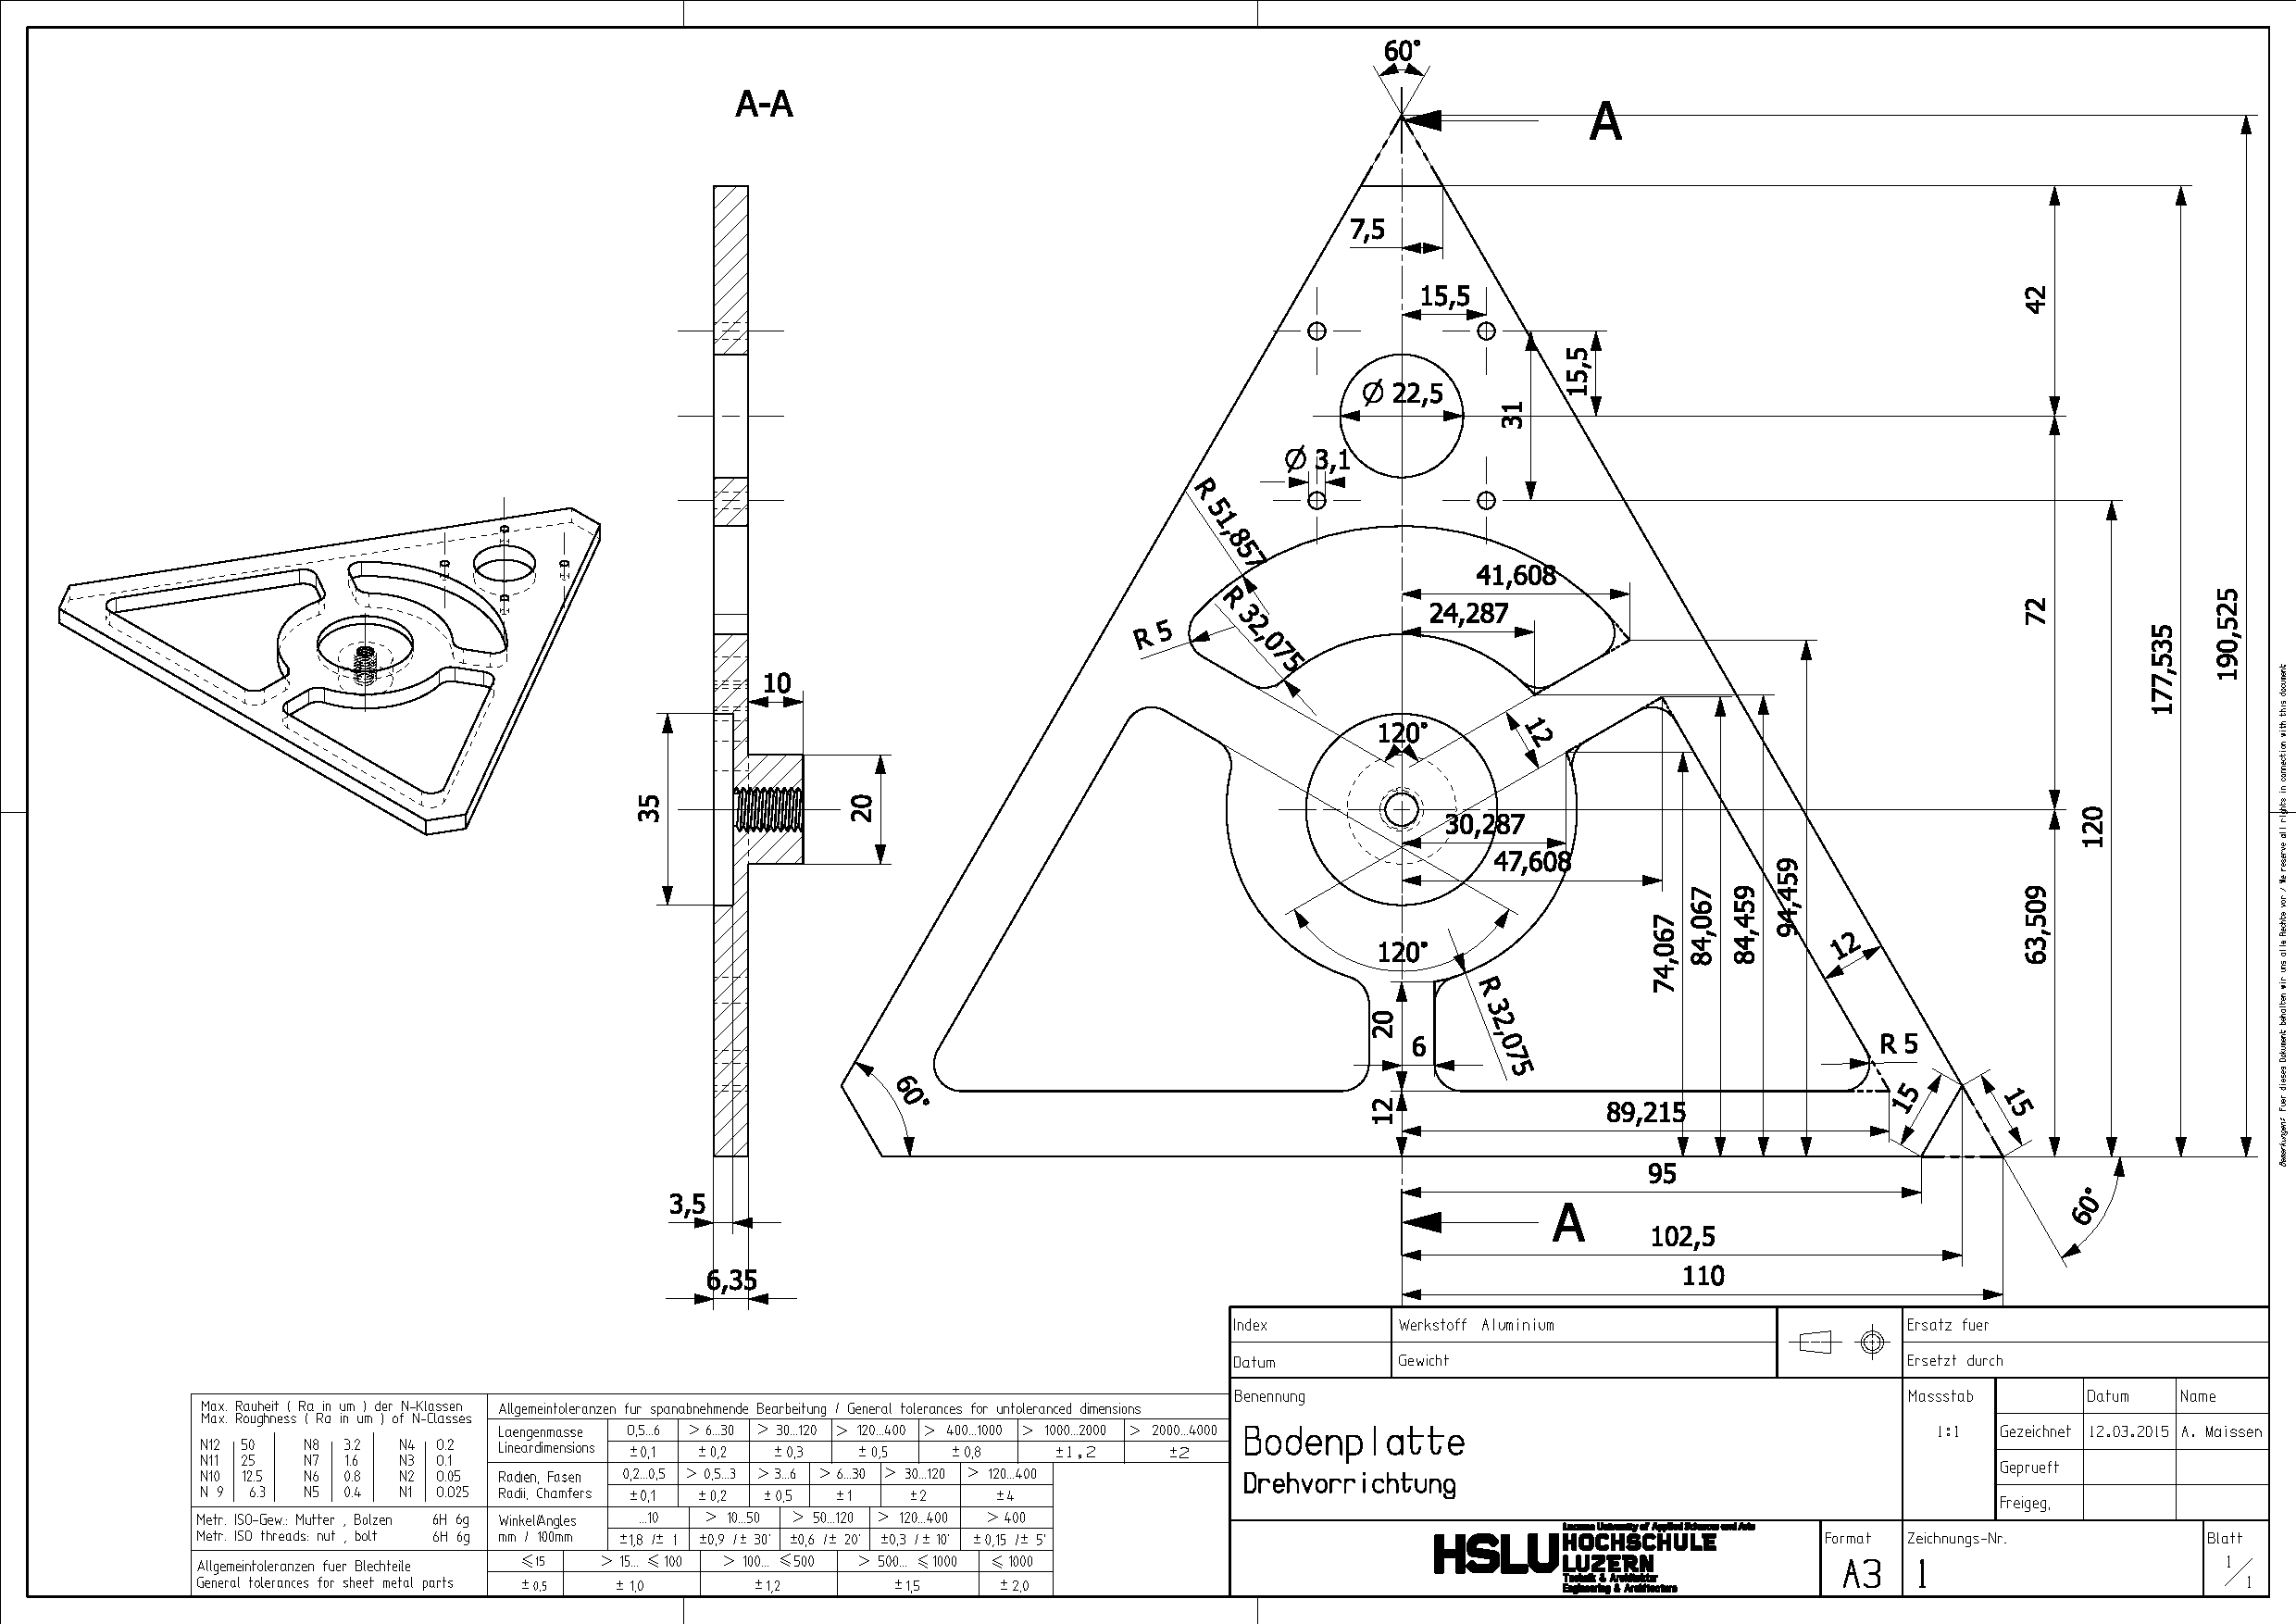
\includegraphics[width=1.0\textwidth]{FotosM/Bild1.pdf}
        \end{column}
    \end{columns}
\end{frame}
\begin{frame}
    \frametitle{Fertigung}
    \begin{columns}
        \begin{column}{0.9\textwidth}
            \centering
            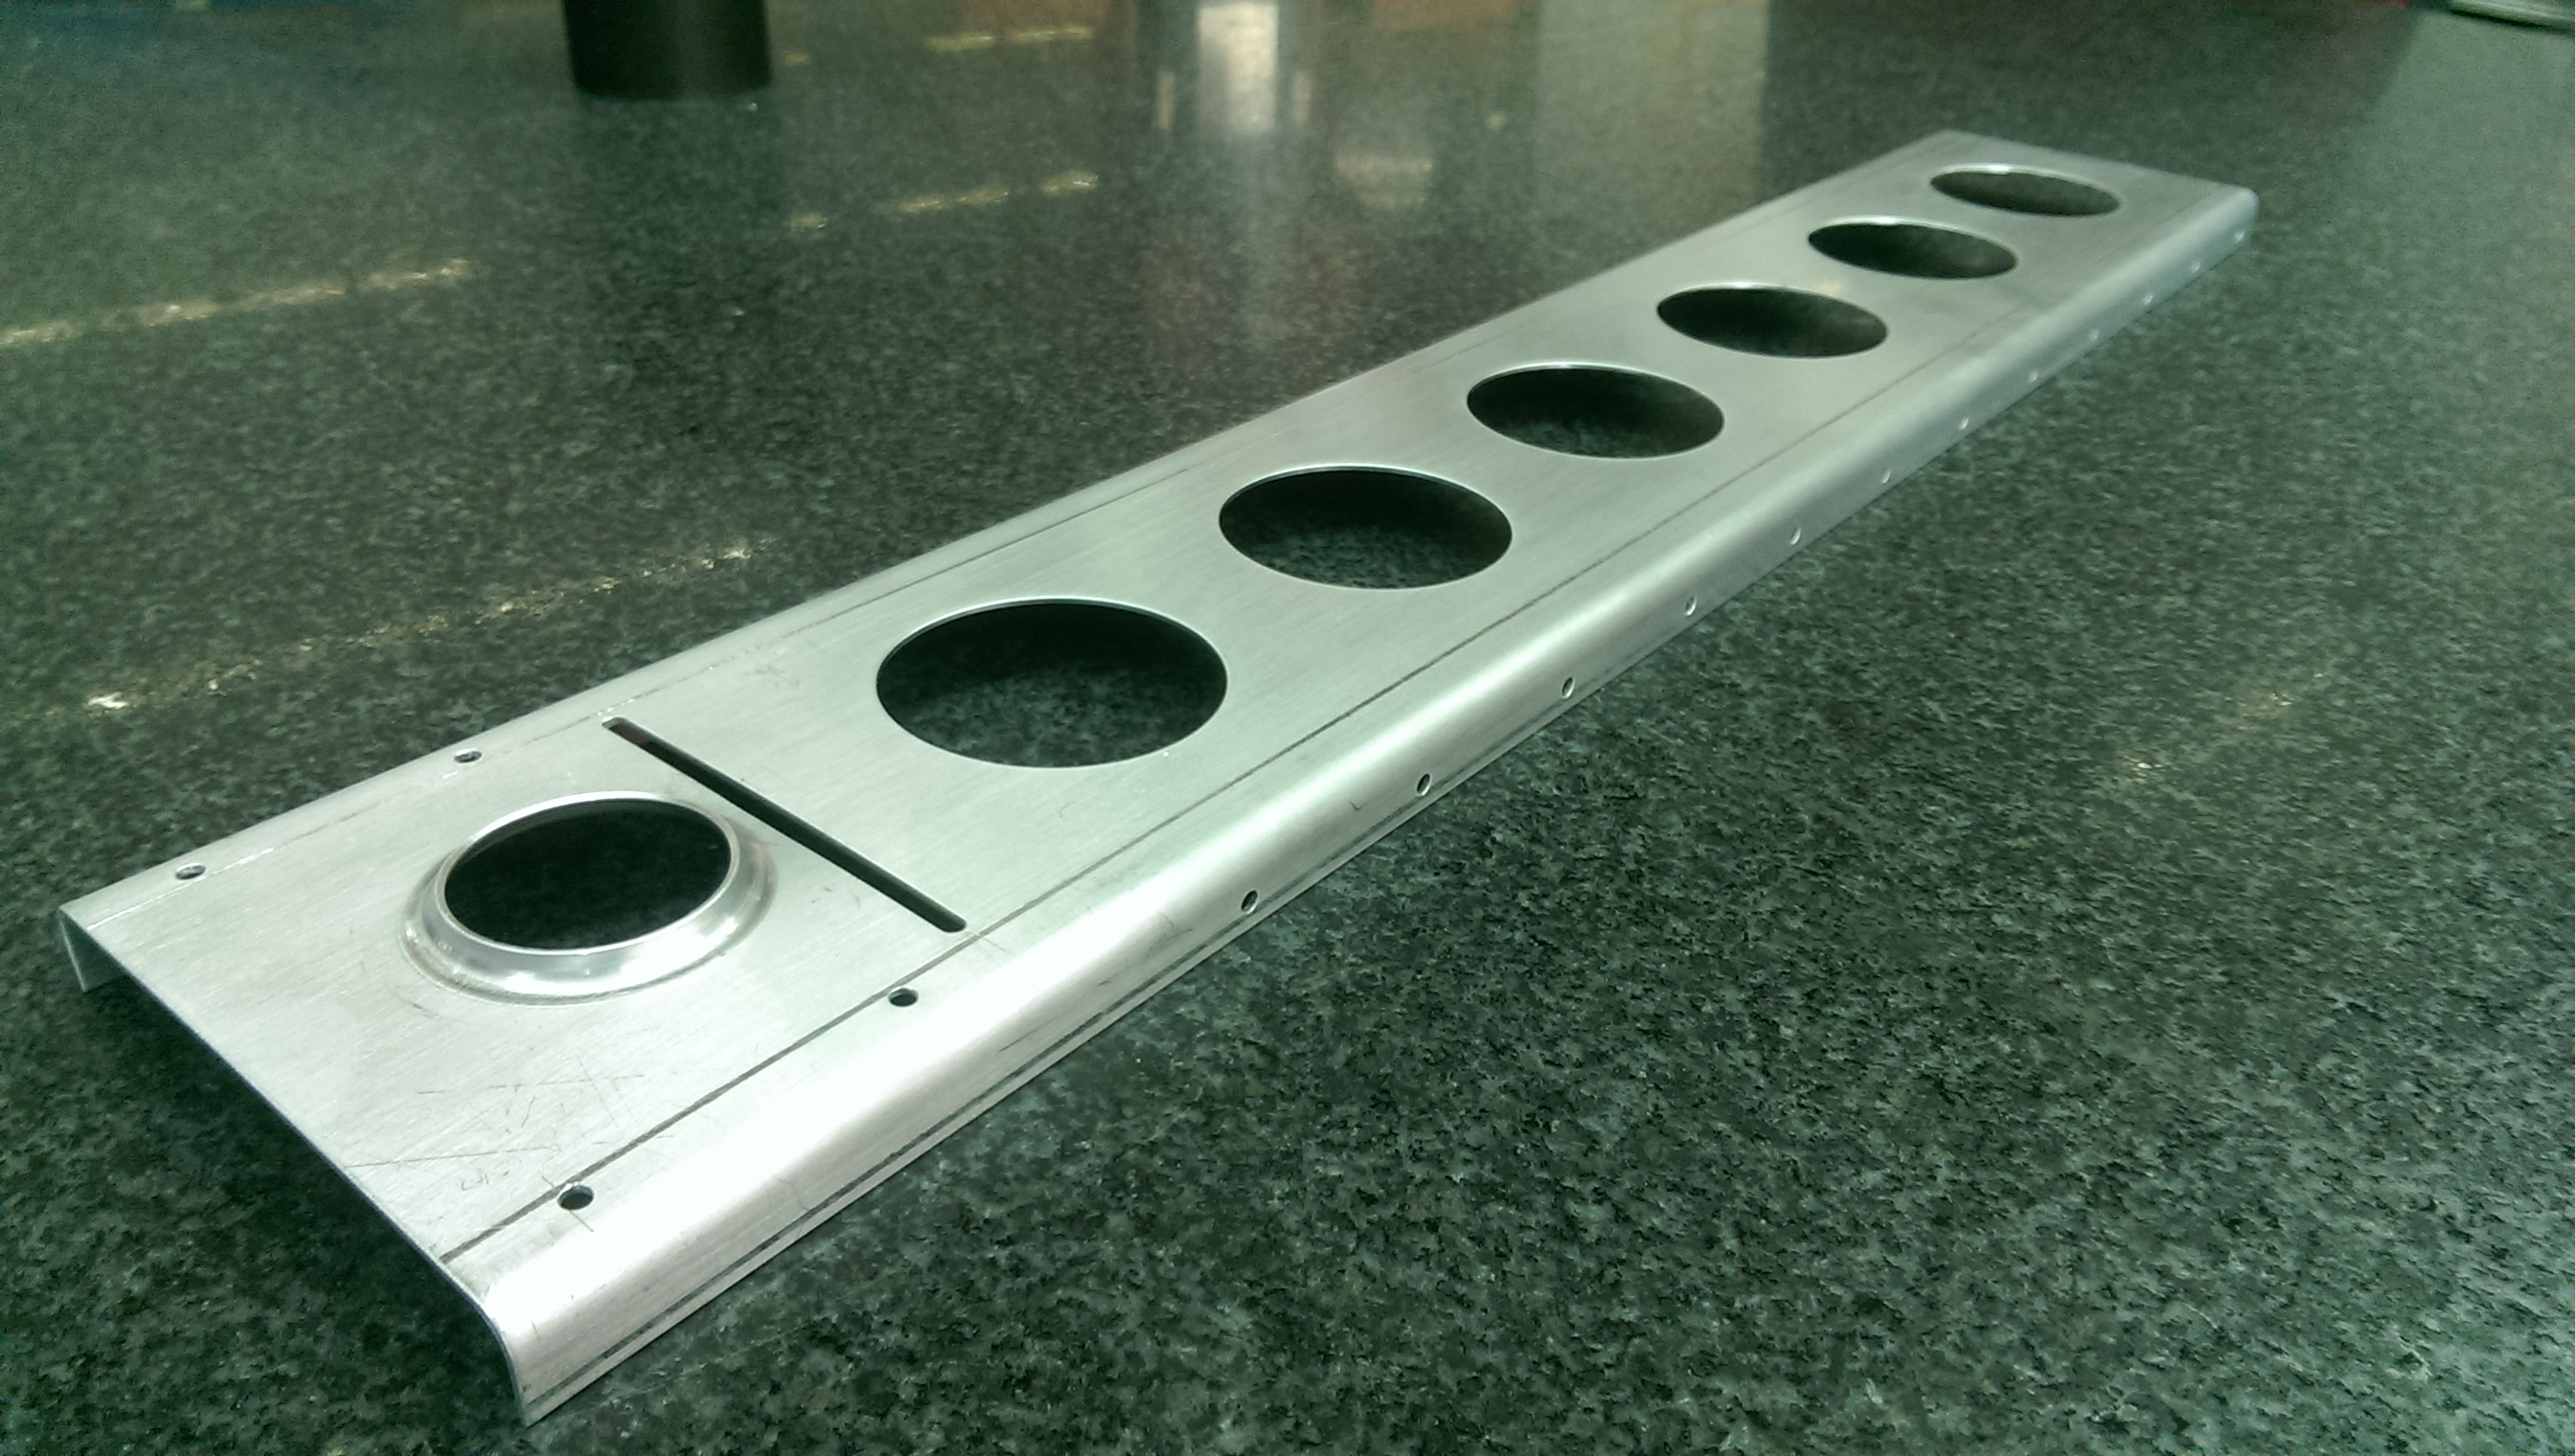
\includegraphics[width=1.0\textwidth]{FotosM/Bild2.jpg}
        \end{column}
    \end{columns}
\end{frame}

%\subsection{Herstellung mechanische Komponenten}
Die konzeptionellen CAD-Zeichnungen werden ab Semesterwoche 2 weiter 
ausgearbeitet, abgewickelt und die Fertigungszeichnungen erstellt. Hierbei 
müssen hauptsächlich Details wie Bohrungen für die Nieten angebracht und 
einige konstruktive Anpassungen vorgenommen werden. 

Ab Semesterwoche 3 können die ersten Teile an der Fräsmaschine im 
Elektrotechniklabor produziert werden, wobei parallel  hierzu die restlichen 
Komponenten am CAD fertiggestellt werden.  Um die gebogenen Innenkanten der 
Aussparungen zu realisieren, werden die gefrästen Blechteile mit einer 
Handpresse und eigens hierfür hergestellten Werkzeugen gefertigt.

In Semesterwoche 4 werden die Grundplatte zur Fertigung an der HSLU in Auftrag 
gegeben.

In Semesterwoche 5 werden zusätzlich einige Teile zum spanenden Herstellen, 
sowie zum 3D-Drucken in Auftrag gegeben. Ebenfalls wird eine 
Rohmaterialbestellung abgegeben.

Die in Auftrag gegebenen Teile können in Semesterwoche 6 abgeholt werden, 
wobei das  Rohmaterial fälschlicherweise aus Stahl, anstatt aus Aluminium, 
bestellt wurde. Eine neue Bestellung des richtigen Rohmaterials wurde abgesetzt.

In Semesterwoche 7 können die bestellten Teile sowie die zum biegen extern in 
Auftrag gegebenen Teile abgeholt werden. Des weiteren wird mit dem Zusammenbau 
der einzelnen Komponenten begonnen. Aufgrund eines beim Biegen entstandenen 
Verzugs einzelner Bauteile und einiger konstruktiver Ungenauigkeiten müssen 
diverse Bohrungen durch feilen nachgebessert werden. Durch Niethefter kann die 
Konstruktion bis zum endgültigen Vernieten aufgebaut werden.

\begin{figure}[h!]          
	\centering             
	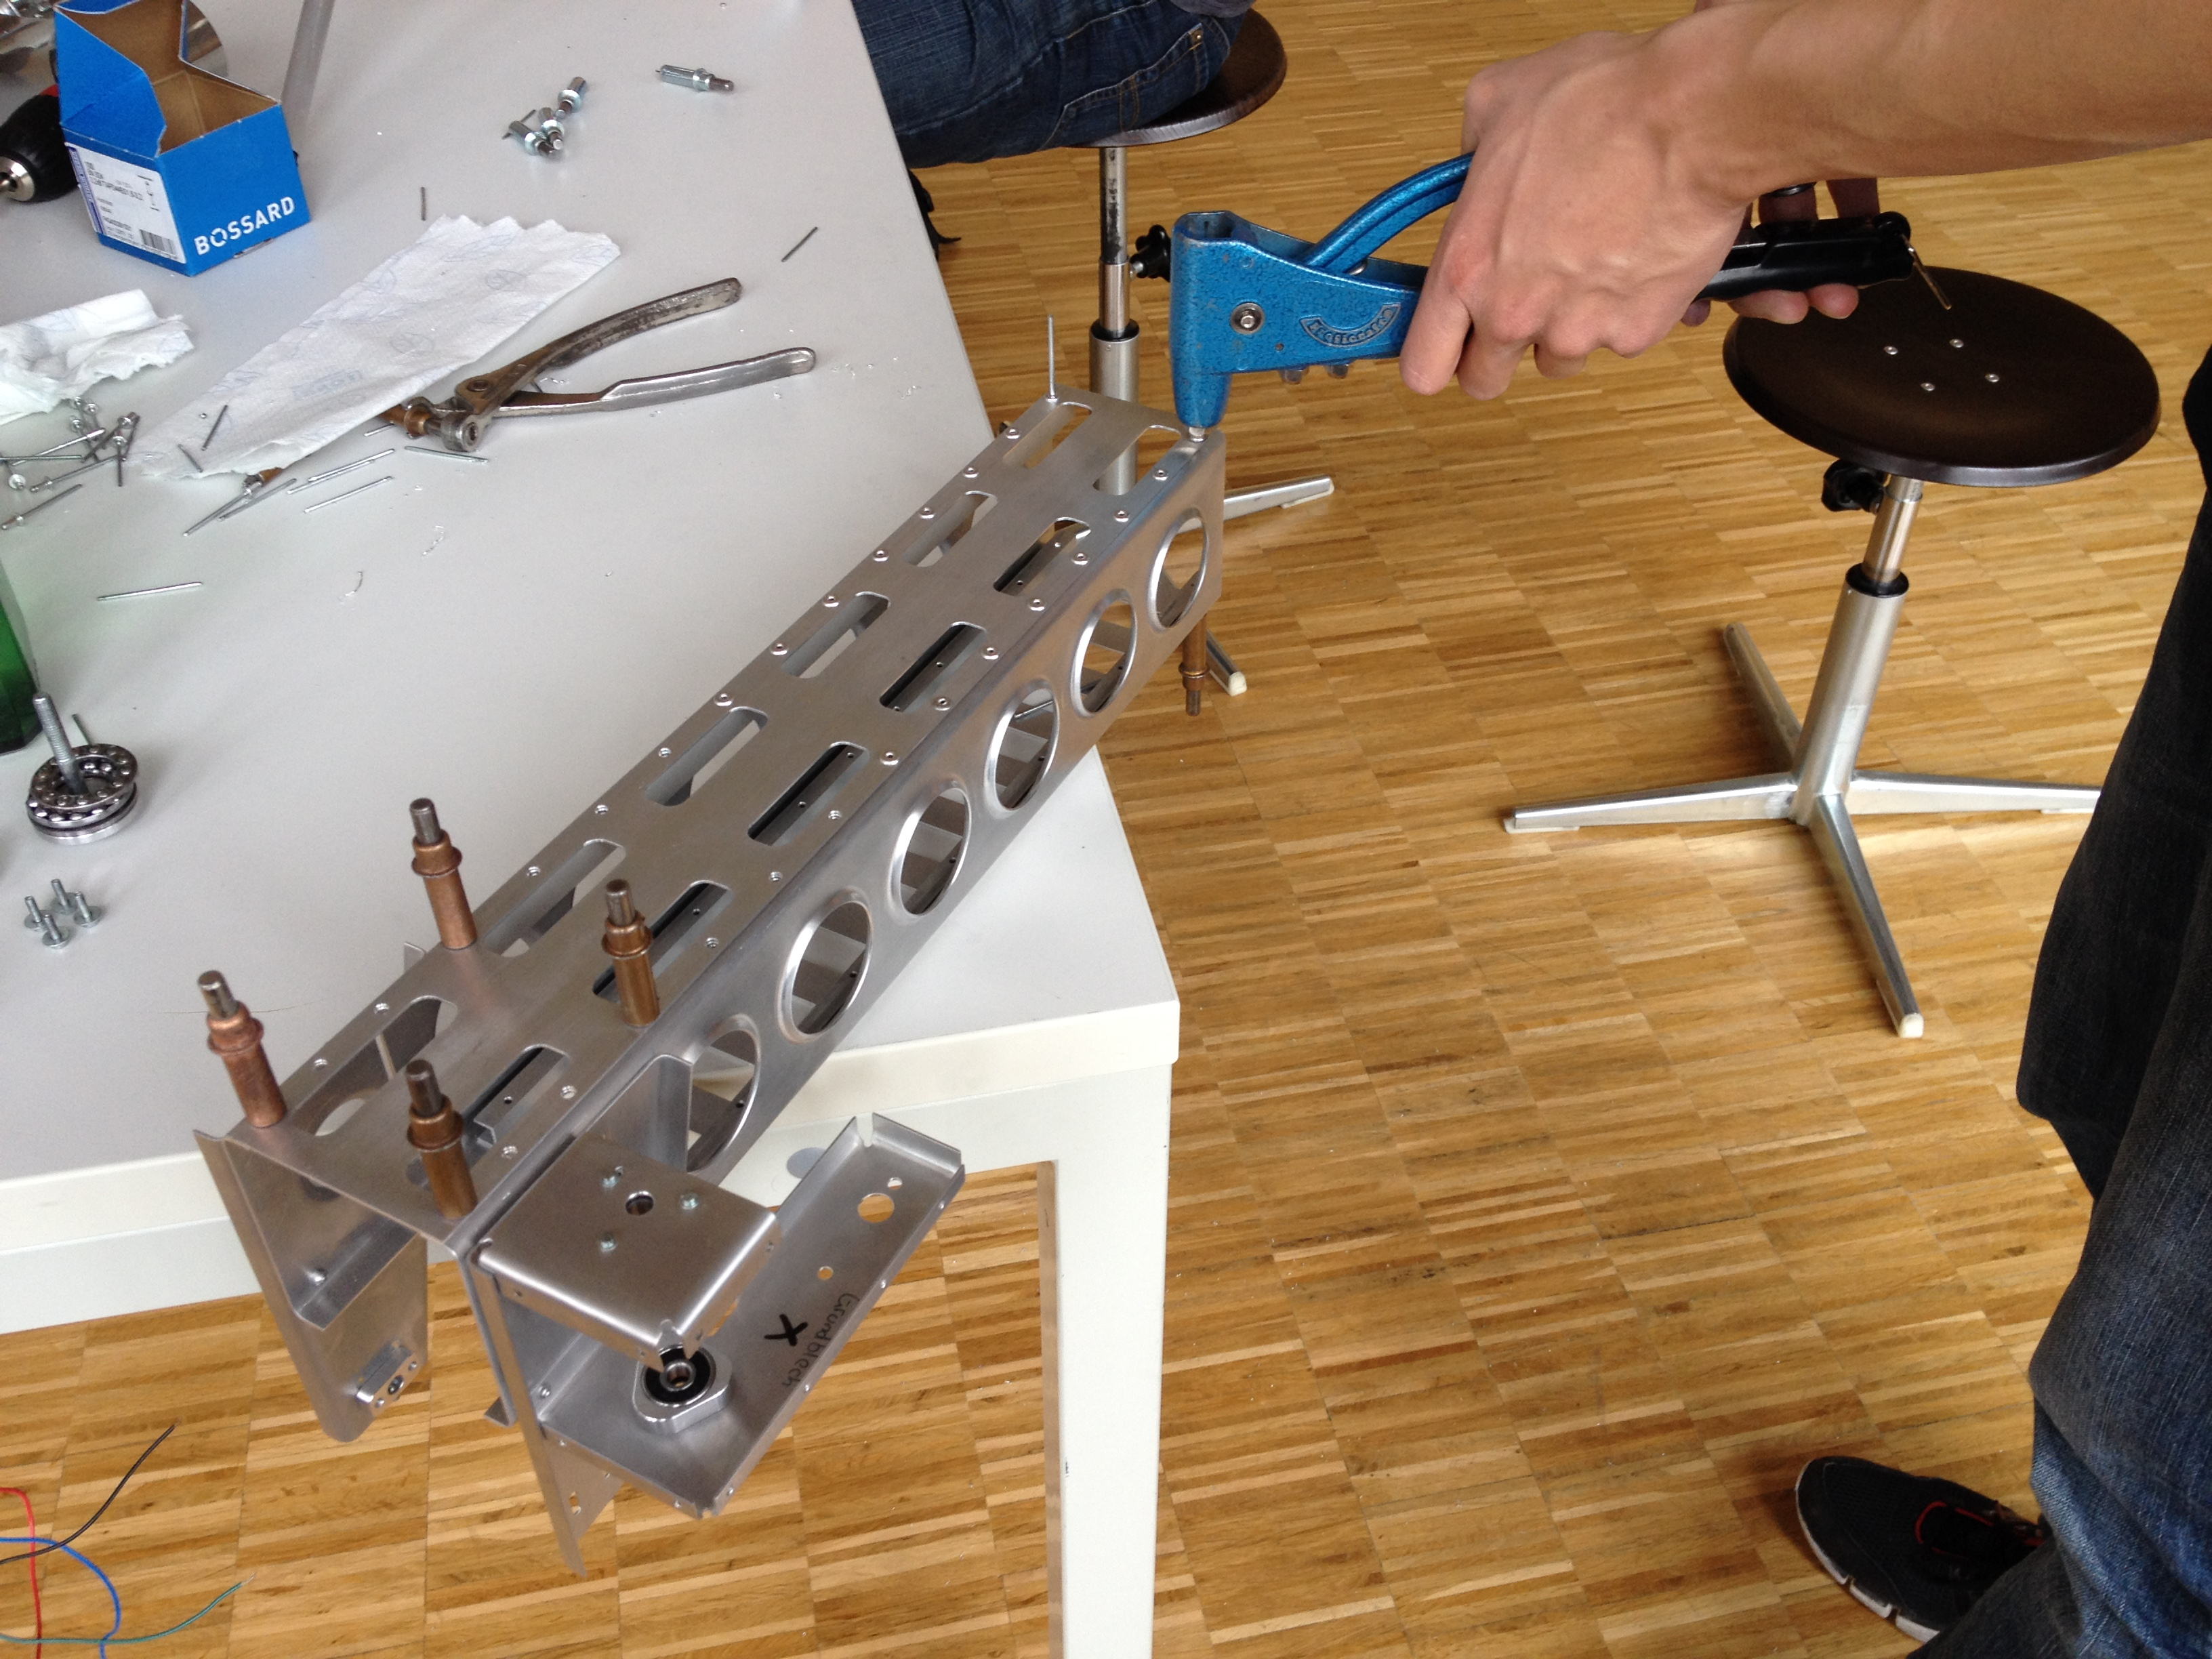
\includegraphics[width=0.5\textwidth]{fig/IMG_2290.JPG}
	\caption{Zusammenbau Balllager}
	\label{fig:Zusammenbau Balllager}        
\end{figure}

\begin{figure}[h!]          
	\centering             
	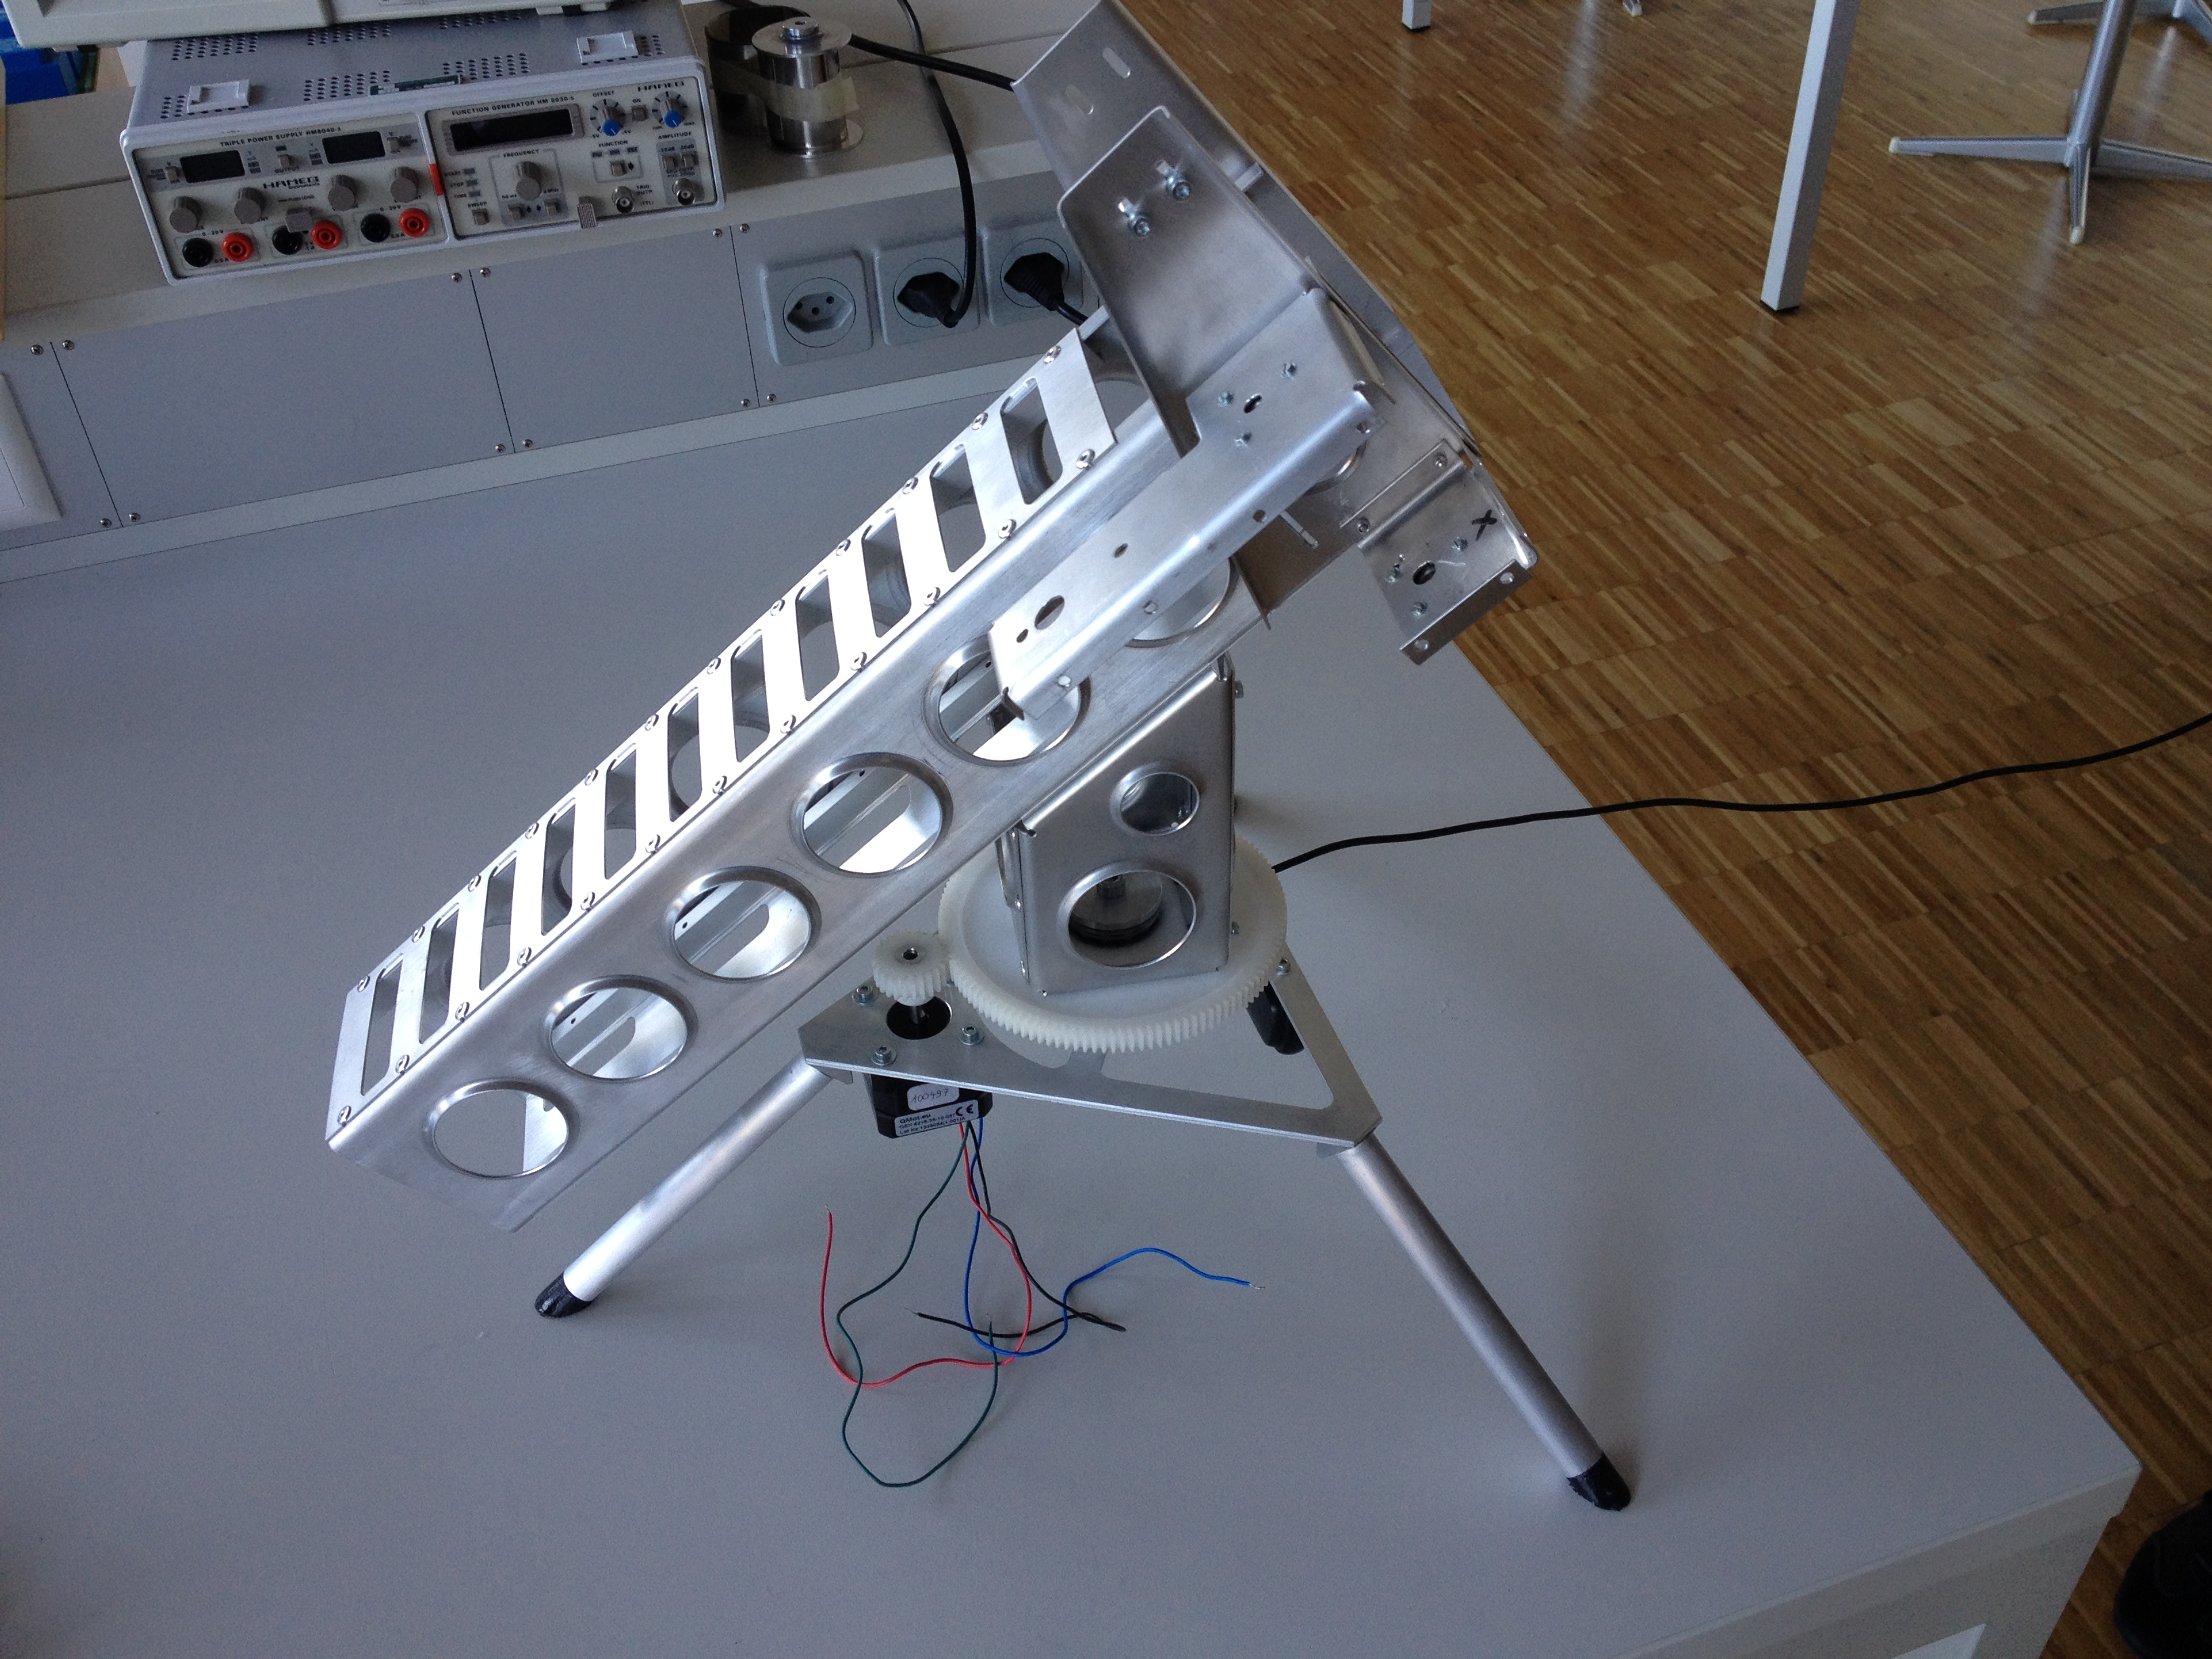
\includegraphics[width=0.5\textwidth]{fig/IMG_2303.JPG}
	\caption{Unvollständiger Aufbau}
	\label{fig:Unvollständiger Aufbau}        
\end{figure}

\paragraph{Nachfolgend werden die speziellen Anpassungen einzelner Komponenten genauer beschrieben:}

\paragraph{Balllager}
Anhand der Erfahrungen erster Testläufe wird entschieden, keine Verstärkung an 
der Unterseite des vorderen Endes anzubringen. Diese Verstärkung hätte eine zu 
starke Durchbiegung des Blechs beim Abschuss der Bälle verhindert.

\paragraph{Ballnachschub}
Beim Zusammenbau wird festgestellt, dass die Welle der Trommel einen zu 
grossen Durchmesser hat und daher mit Hilfe einer Handbohrmaschine und 
gewöhnlichem Schleifpapier auf das gewünschte Mass geschliffen werden muss.

\paragraph{Drehvorrichtung}
Um weiteres Gewicht einzusparen wird die bereits hergestellte Grundplatte auf die halbe Höhe überfräst.

\begin{figure}[h!]          
	\centering             
	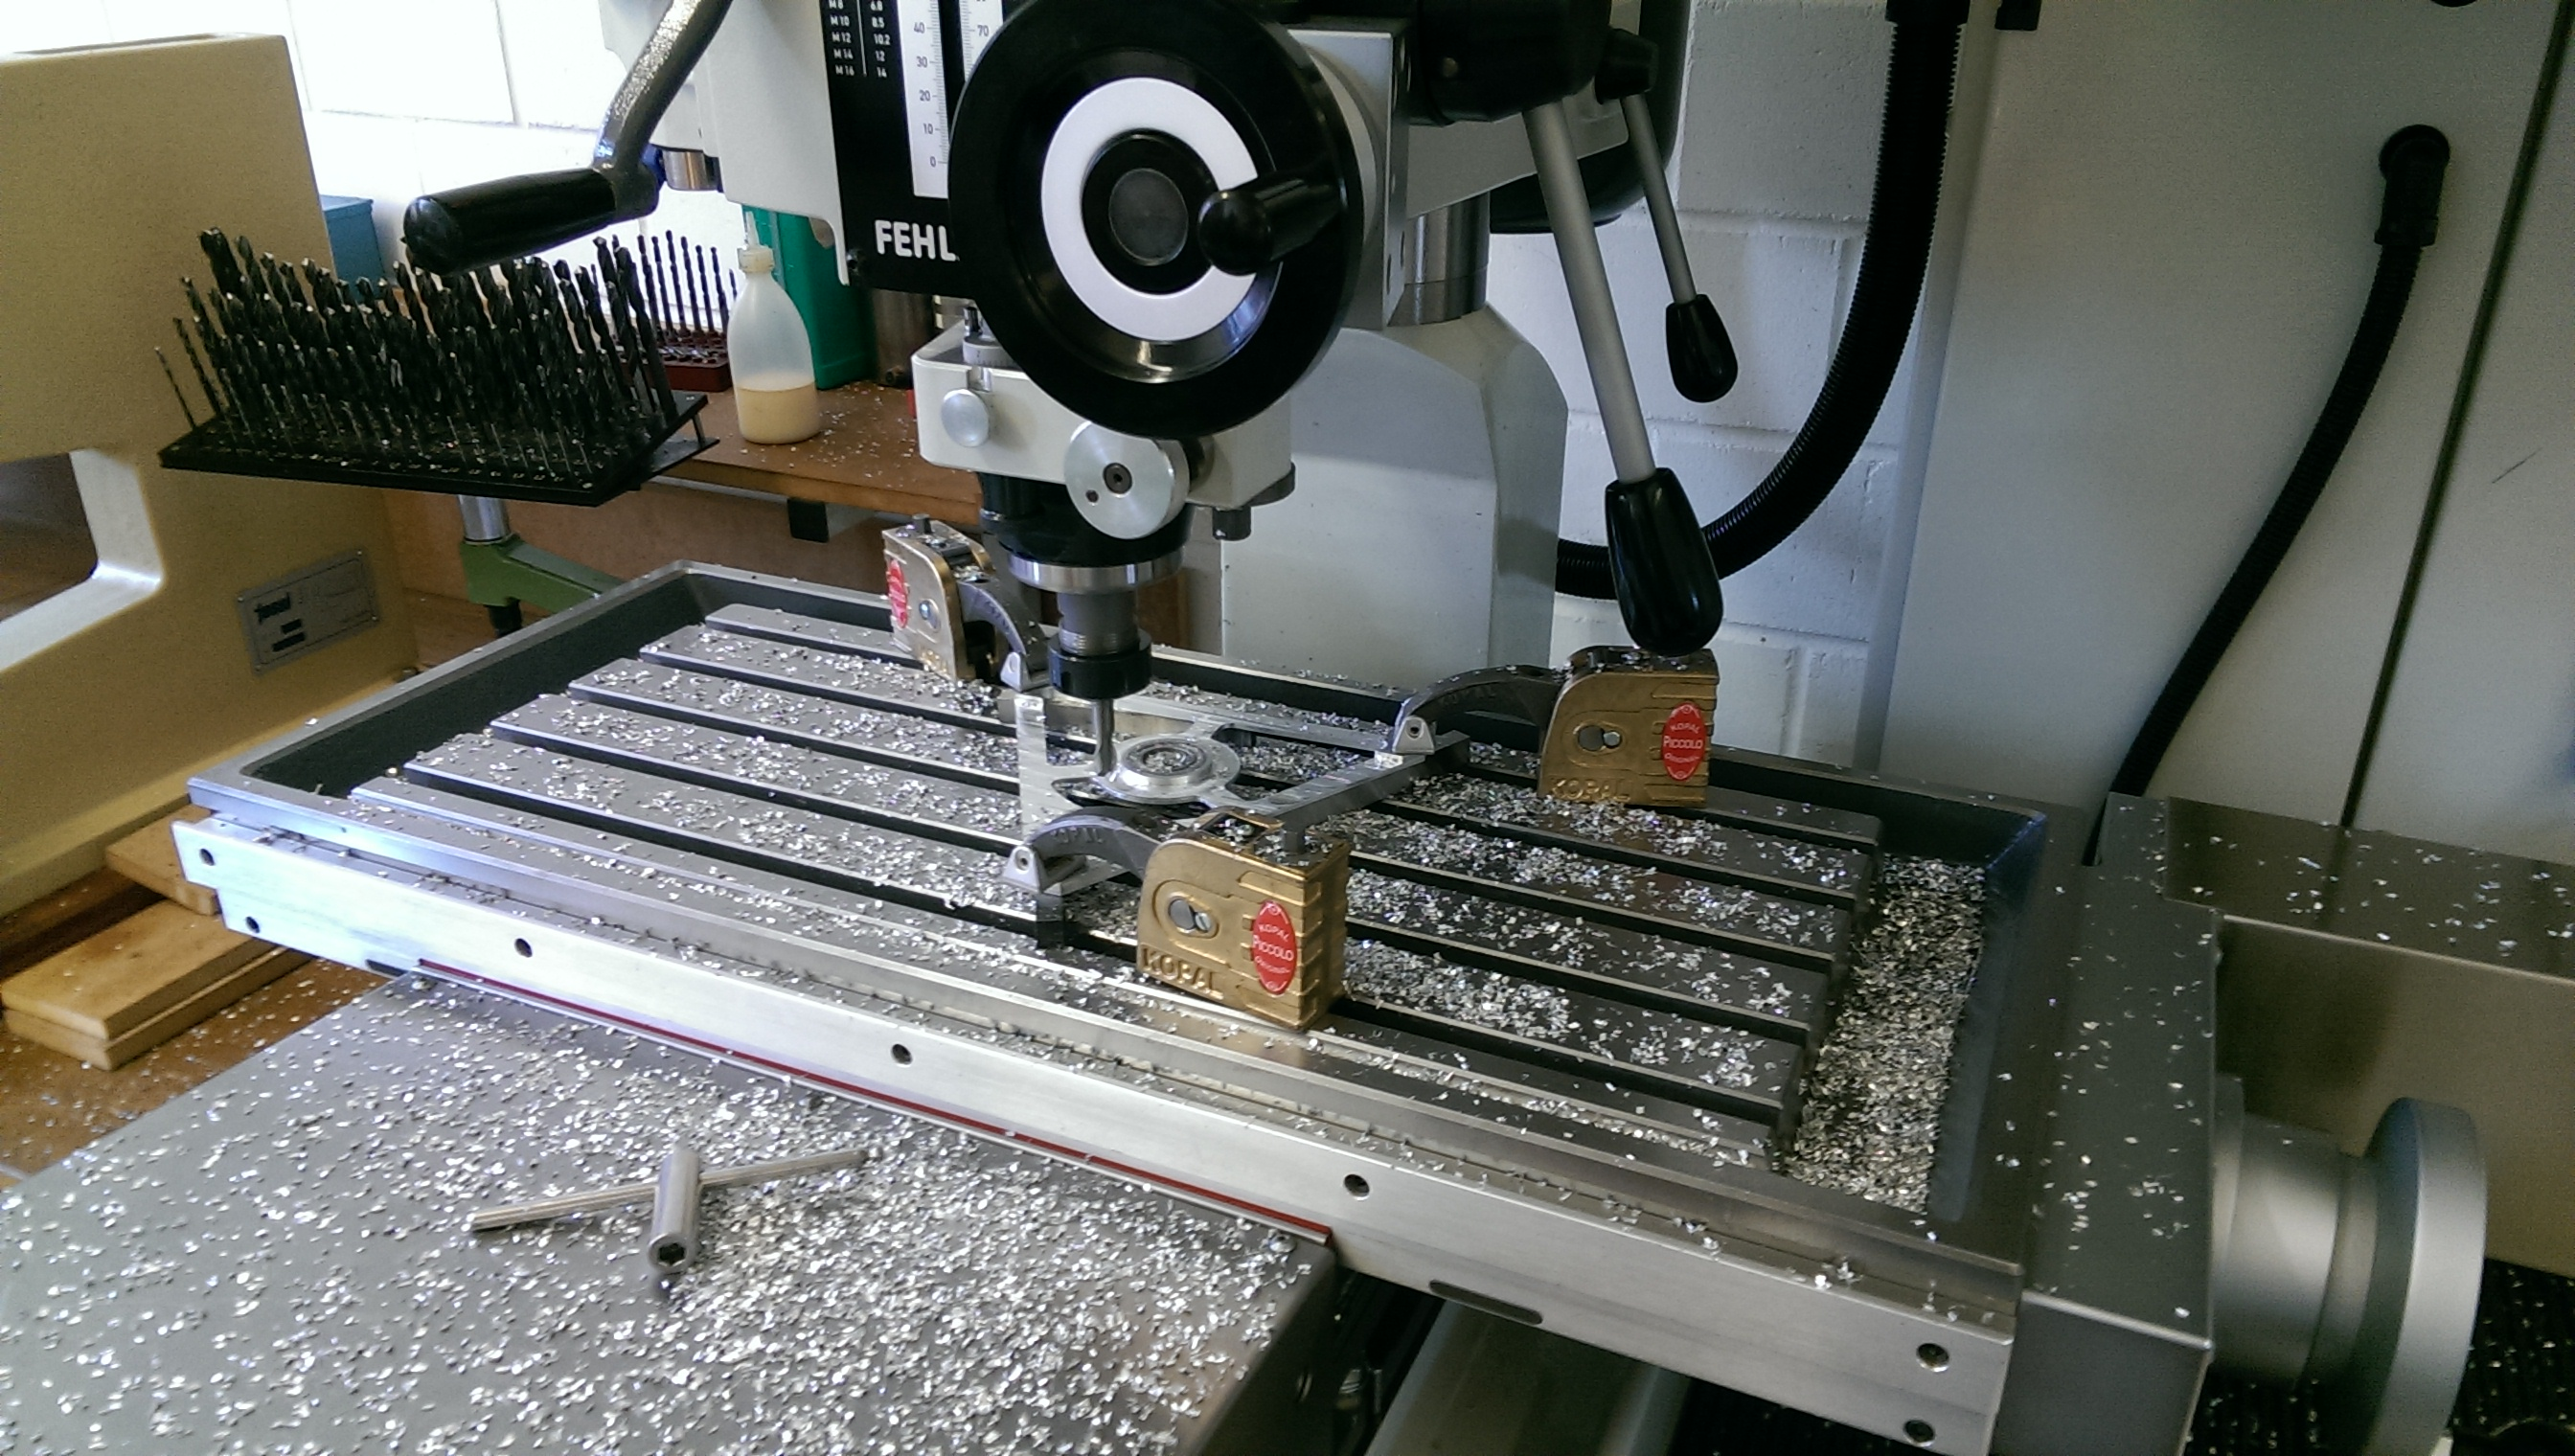
\includegraphics[width=0.5\textwidth]{fig/IMAG0357.jpg}
	\caption{Überfräsen der Grundplatte}
	\label{fig:Grundplatte fräsen}        
\end{figure}

\paragraph{Motor}
Zunächst wird der Rotor des Motors auf einer CNC-Fräse gefräst und der 
Stahlring eingepresst. Anschliessend werden sämtliche Magnete von Hand 
eingesetzt und mit Zweikomponentenklebstoff befestigt. Die Statorbleche für 
den Motor stammen aus Floppydisk-Laufwerken. Dazu müssen für einen Motor die 
Statoren aus zwei Laufwerken ausgebaut werden. Anschliessend werden die 
bestehenden Wicklungen von den Statoren entfernt. Die Statorbleche und die 
Kunststoffisolatoren werden für den neuen Motor weiterverwendet. Dazu werden 
die Statorbleche aus zwei Motoren aufeinandergelegt und mit der Halterung 
verschraubt. Anschliessend wird der Stator mit neuem Kupferlackdraht 
bewickelt. Nach dem Bewickeln und fixieren der Wicklungen wird der Stator 
passend auf den Durchmesser des Rotors abgedreht. Danach kann der Stator auf 
der passenden Aufnahme befestigt und der Motor zusammengesetzt werden. 
\begin{center}
    \begin{minipage}[c]{0.2\textwidth}
        Bild Floppy (2759)
    \end{minipage}
    \begin{minipage}[c]{0.1\textwidth}
        \Huge$\Rightarrow$
    \end{minipage}
    \begin{minipage}[c]{0.2\textwidth}
        Stator leer (???)
    \end{minipage}
    \begin{minipage}[c]{0.1\textwidth}
        \Huge$\Rightarrow$
    \end{minipage}
    \begin{minipage}[c]{0.2\textwidth}
        Stator bewickelt (2816 / 2751)
    \end{minipage}
\end{center}

Beim Zusammenbau wird bemerkt, dass die Langlöcher der Motorenhalterung zu kurz ausgeführt wurden um einen guten Anpressdruck der Bälle zu ermöglichen. Daher werden diese durch feilen verlängert.

\paragraph{Turm}
Die Muttern der Wartungsklappe werden auf der Innenseite des Turms mit Zweikomponentenklebstoff 
angebracht. 

\begin{figure}[h!]          
	\centering             
	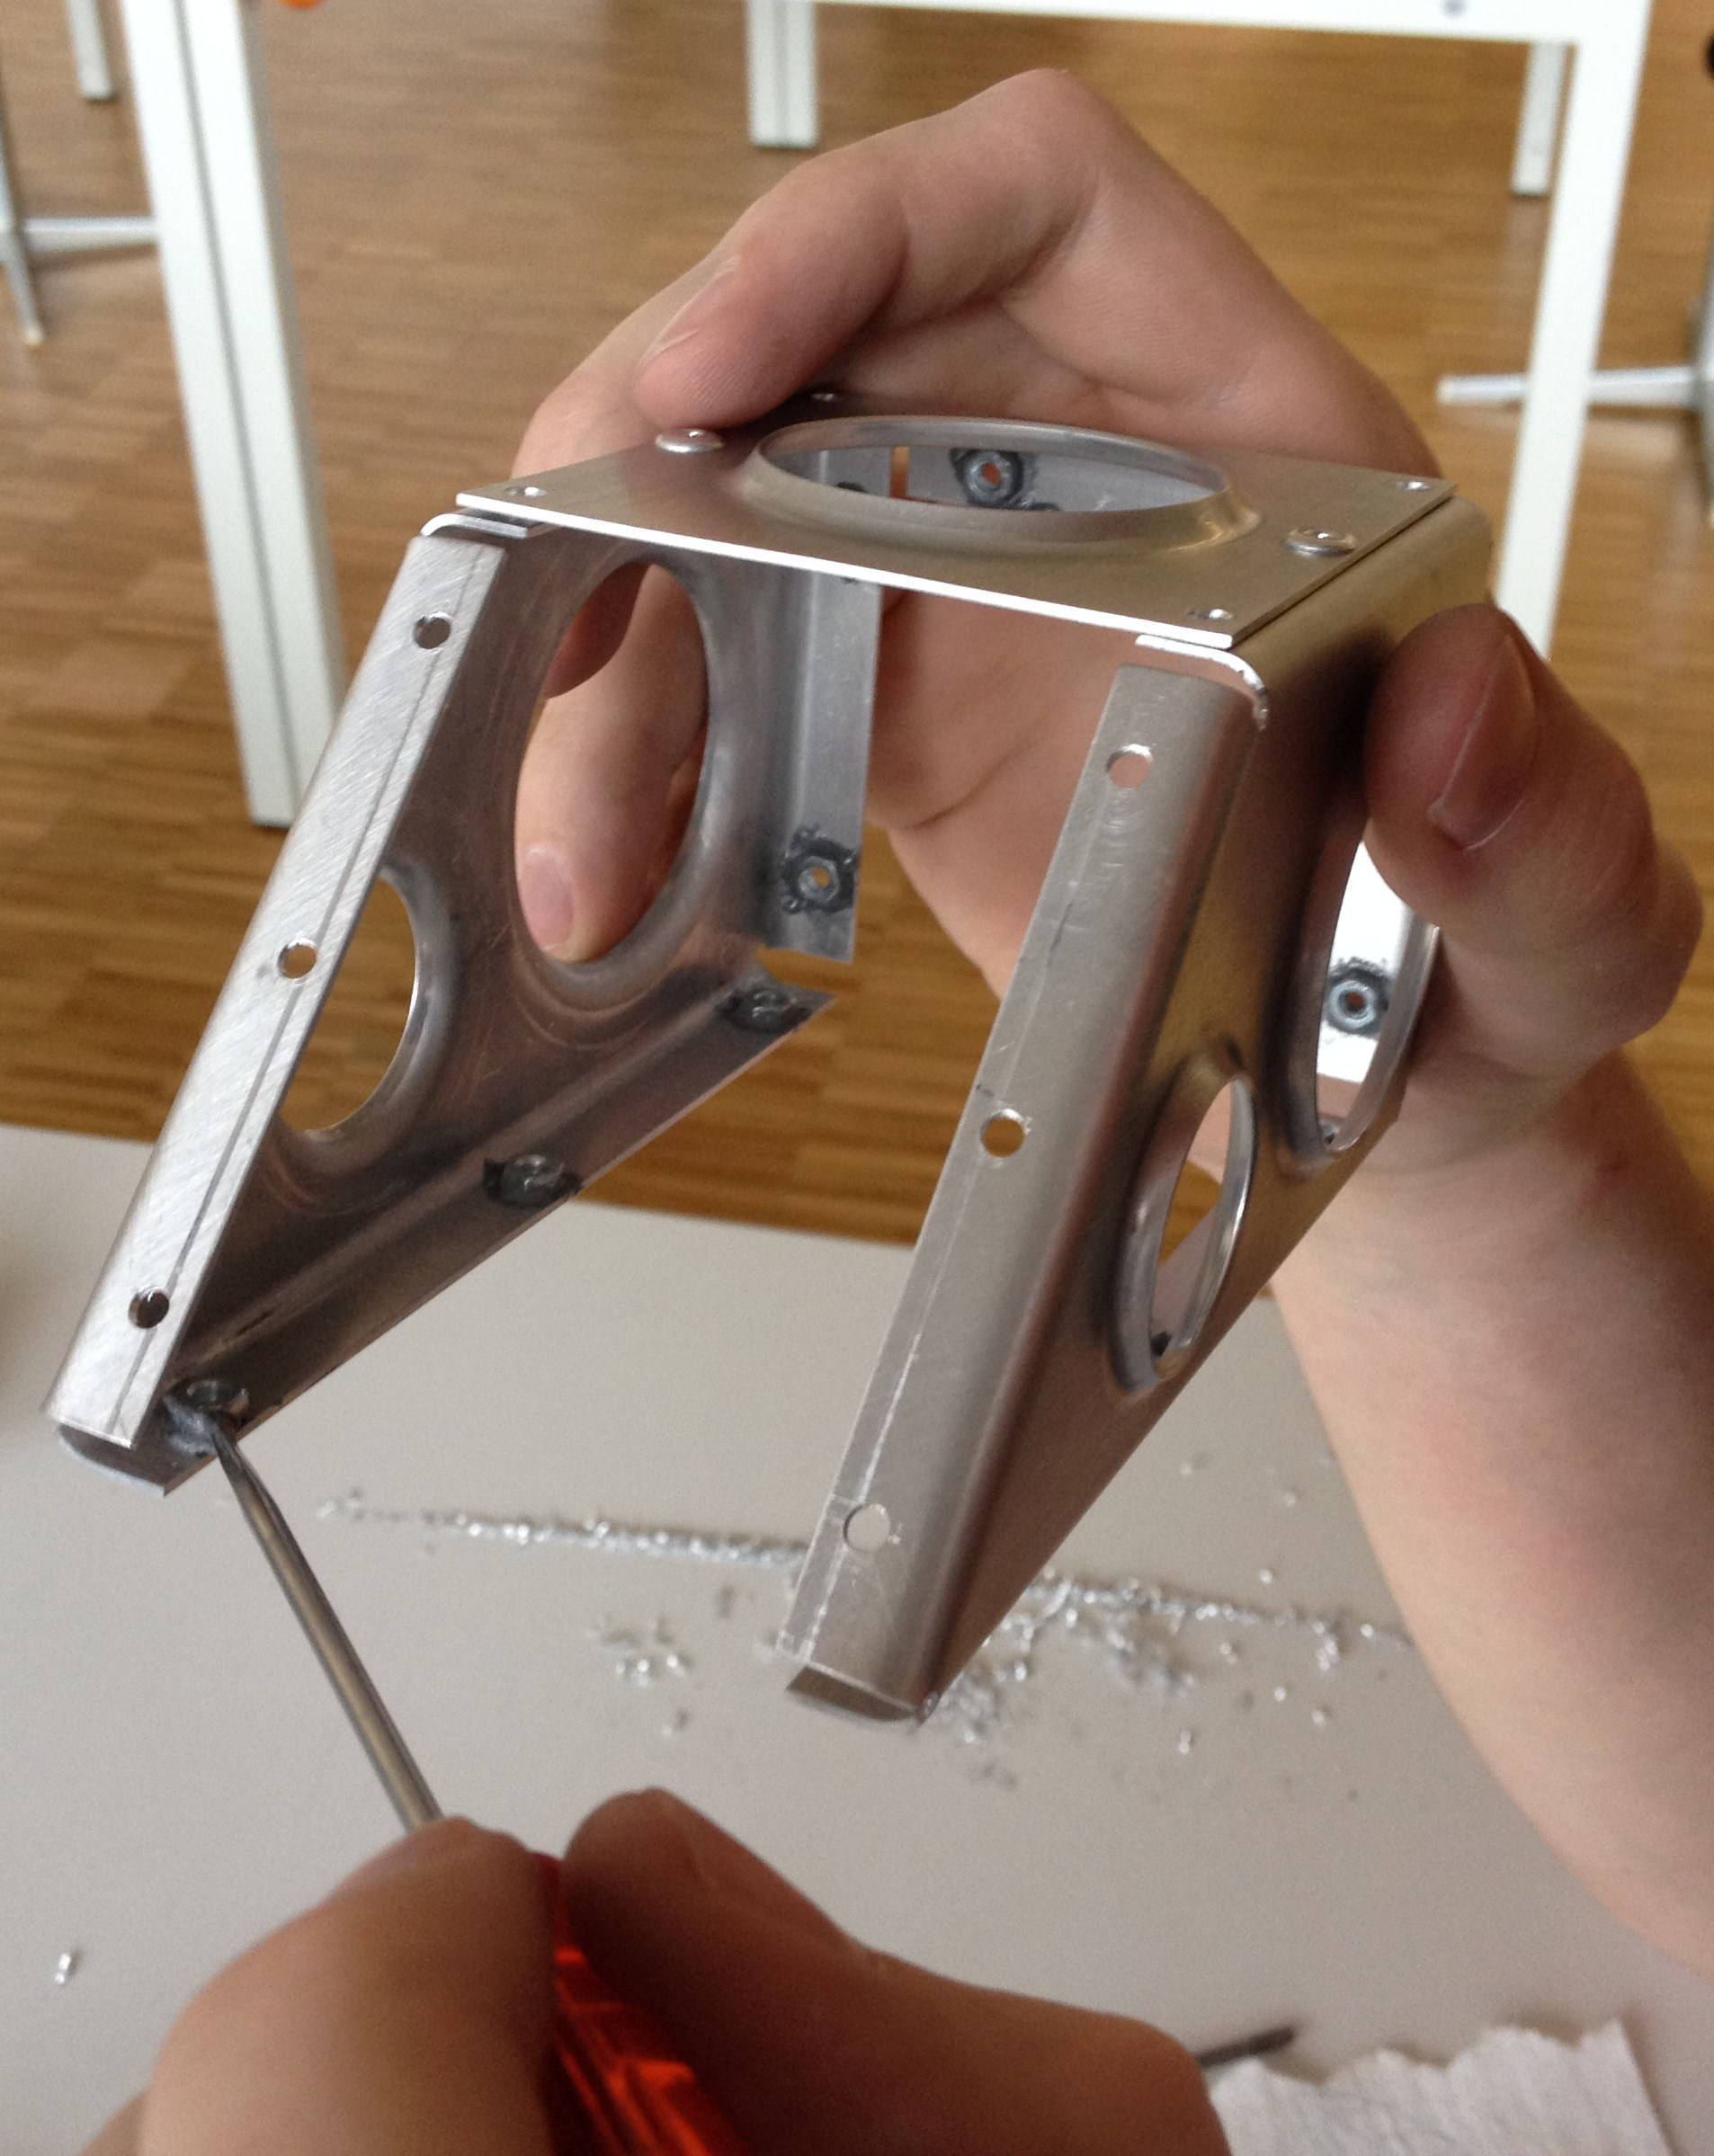
\includegraphics[width=0.3\textwidth]{fig/IMG_2292.JPG}
	\caption{Kleben der Muttern}
	\label{fig:Muttern Kleben}        
\end{figure}



\subsection{Korberkennung}
\begin{frame}
    \frametitle{Kamera}
    \begin{columns}
        \begin{column}{0.9\textwidth}
            \centering
            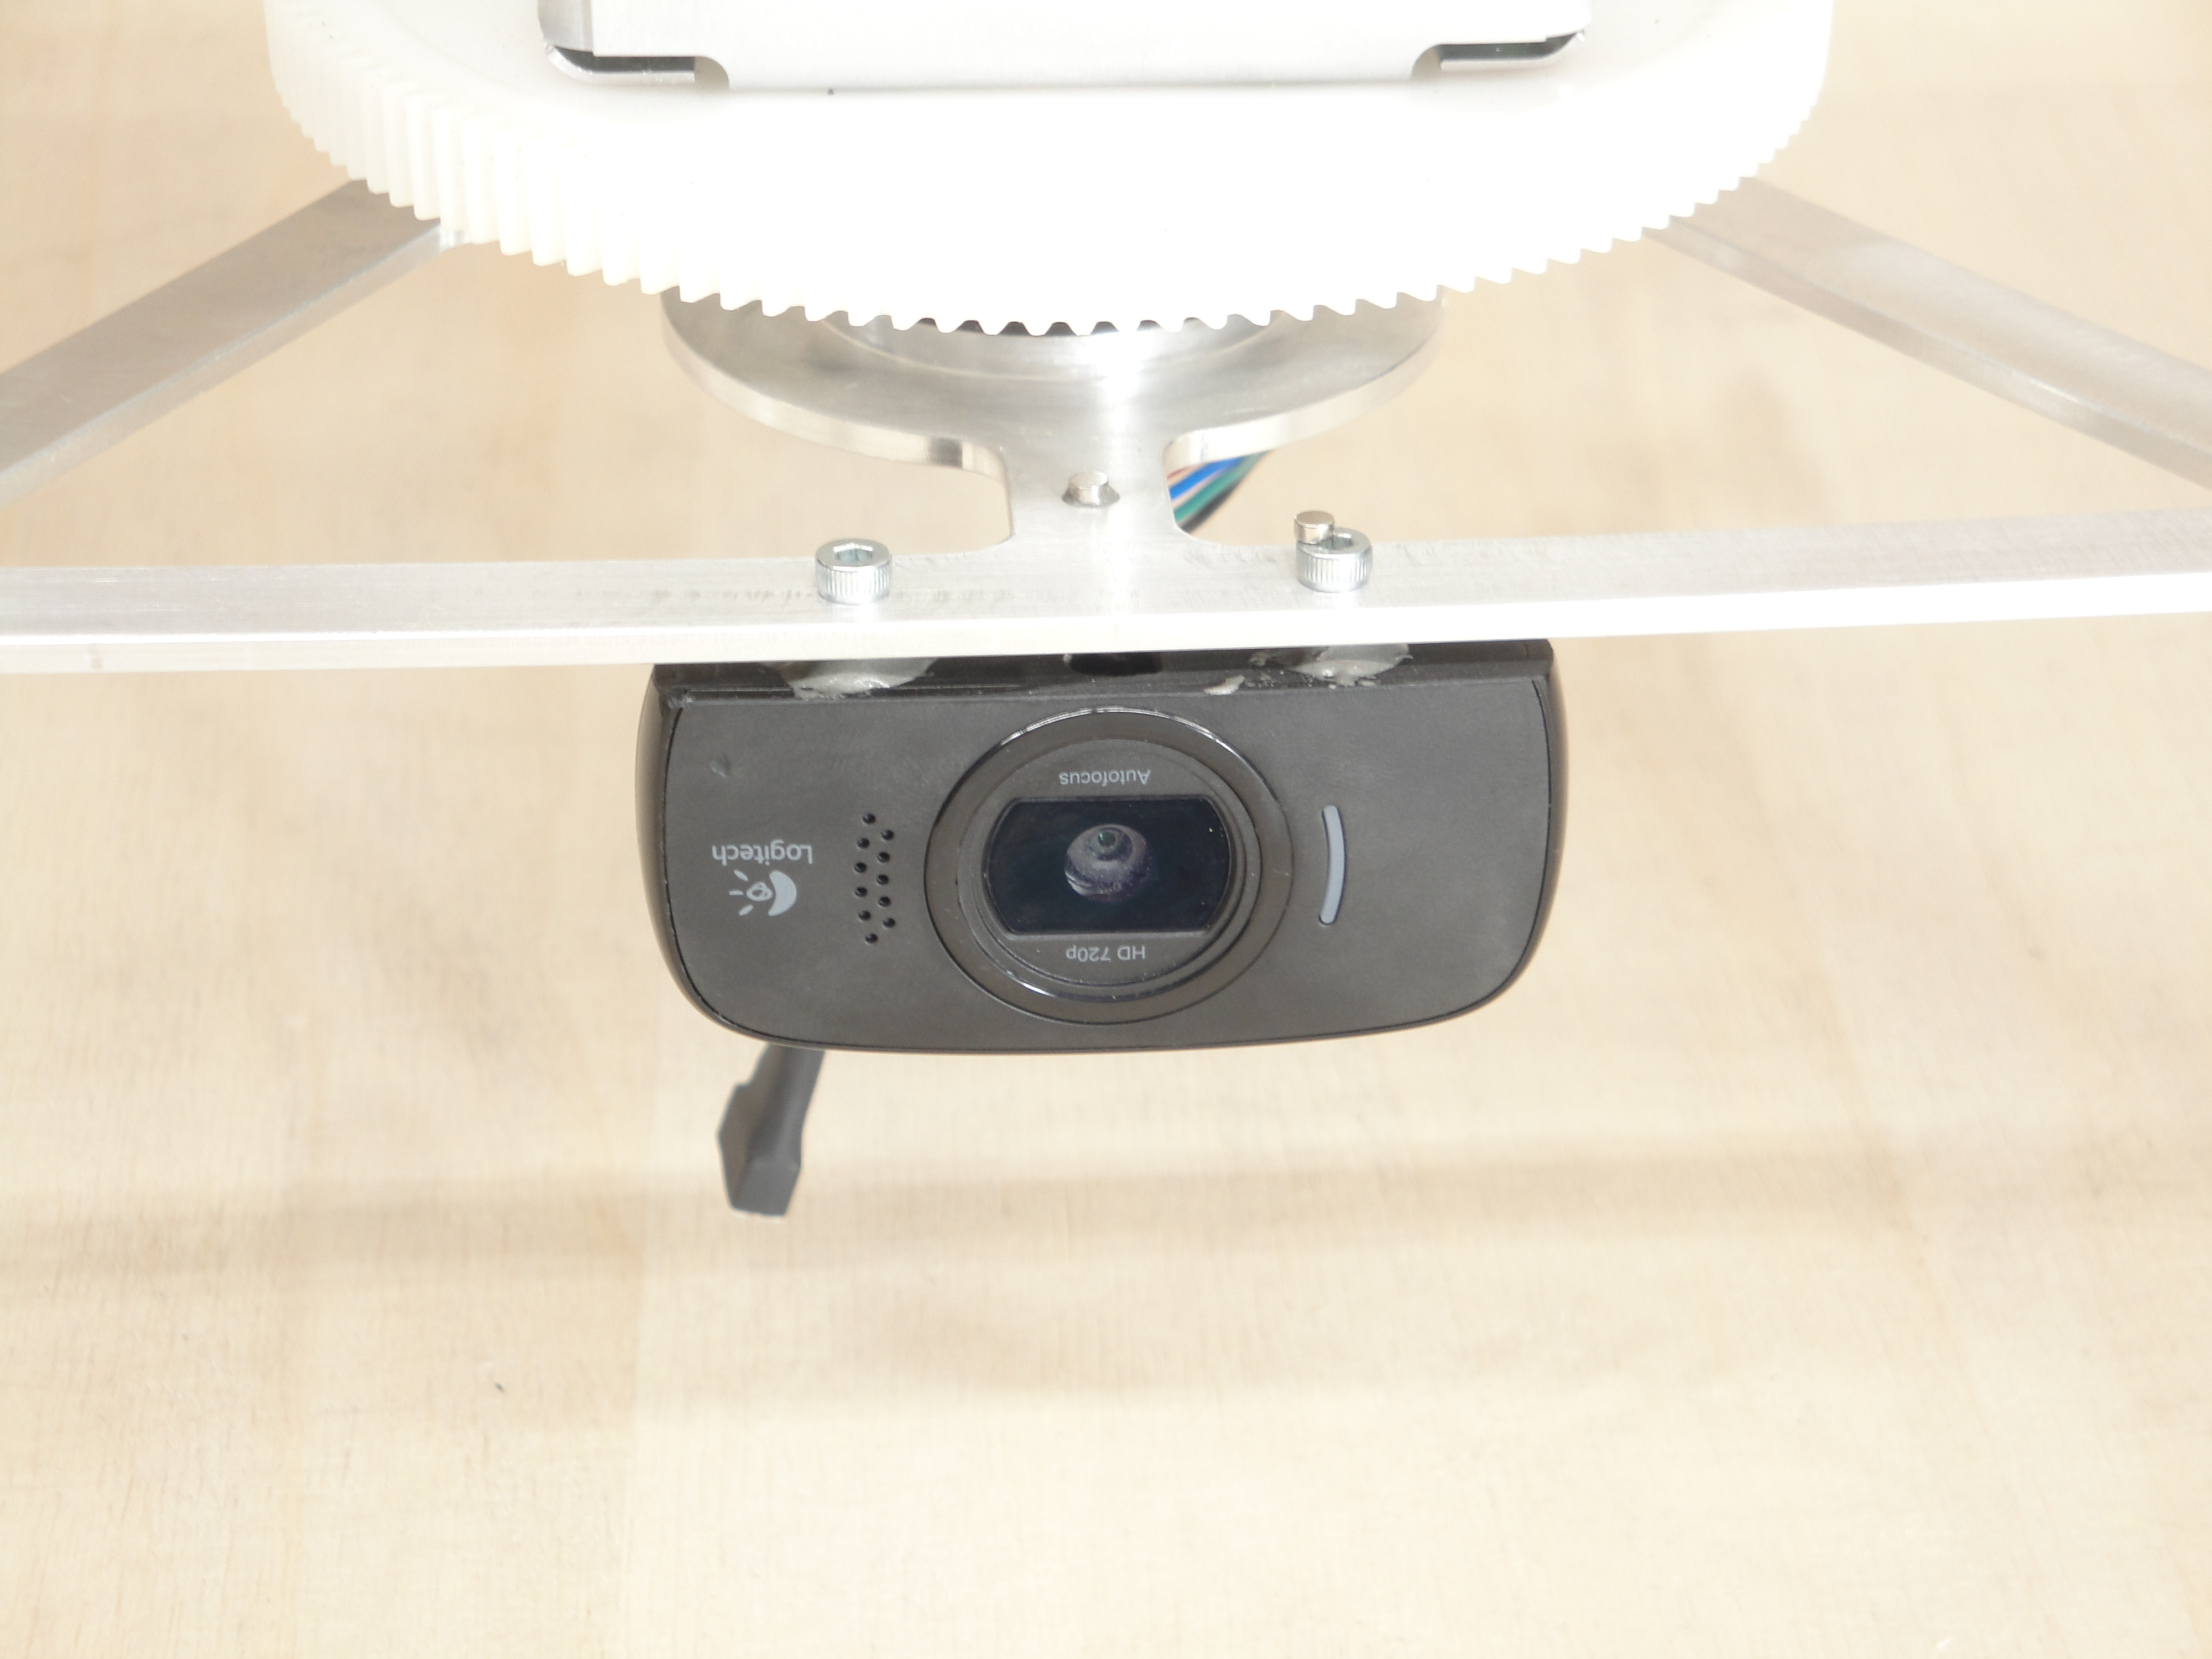
\includegraphics[width=1.0\textwidth]{../doc/fig/DSC02993.JPG}
        \end{column}
    \end{columns}
\end{frame}

\begin{frame}
    \frametitle{Korberkennung}
    \framesubtitle{Korberkennung}
    \begin{columns}
        \begin{column}{0.4\textwidth}
            \begin{block}{Korberkennung}
                \begin{itemize}
                    \item Kamera
                    \item OpenCV
                \end{itemize}
            \end{block}
        \end{column}
        \begin{column}{0.6\textwidth}
            \centering
            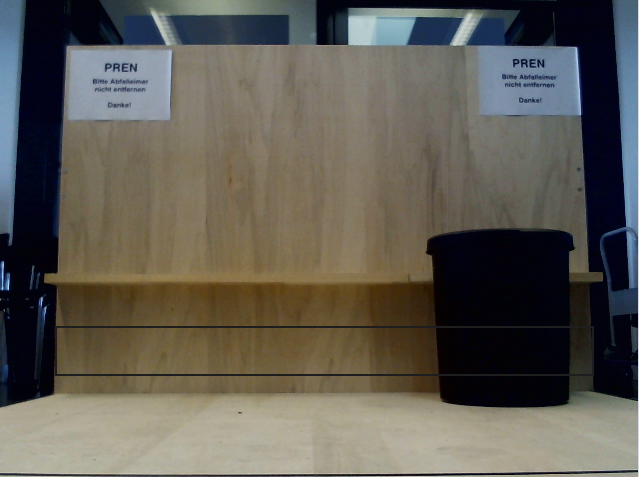
\includegraphics[width=1.0\textwidth]{../doc/fig/BildMitKorb_markiert.png}
        \end{column}
    \end{columns}
\end{frame}


\begin{frame}
    \frametitle{Ablauf Korberkennung}
    \framesubtitle{Ablauf Korberkennung}
    \begin{columns}
        \column{0.6\textwidth}
            \centering
            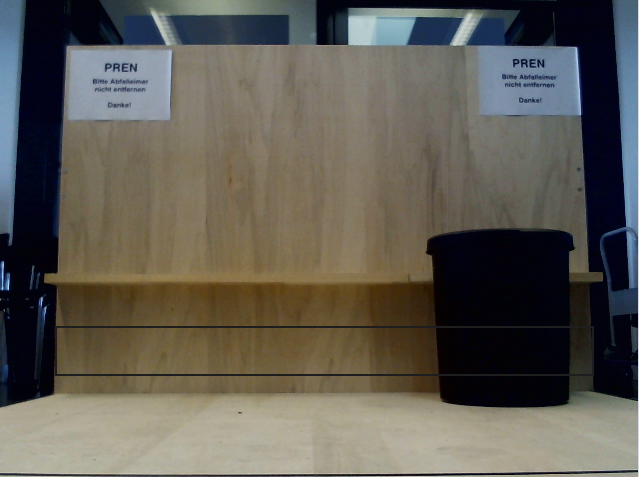
\includegraphics[width=1.0\textwidth, trim=0 40 0 120, clip=true]{../doc/fig/BildMitKorb_markiert.png}
            \rule{0pt}{5pt}
            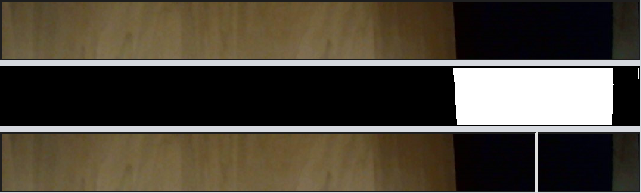
\includegraphics[width=1\textwidth]{../doc/fig/Korberkennung_Schritte.png}
    \end{columns}
\end{frame}


\subsection{Ausrichtung}
\begin{frame}
    \frametitle{Kommunikation}
    \begin{columns}
        \begin{column}{1\textwidth}
            \centering
            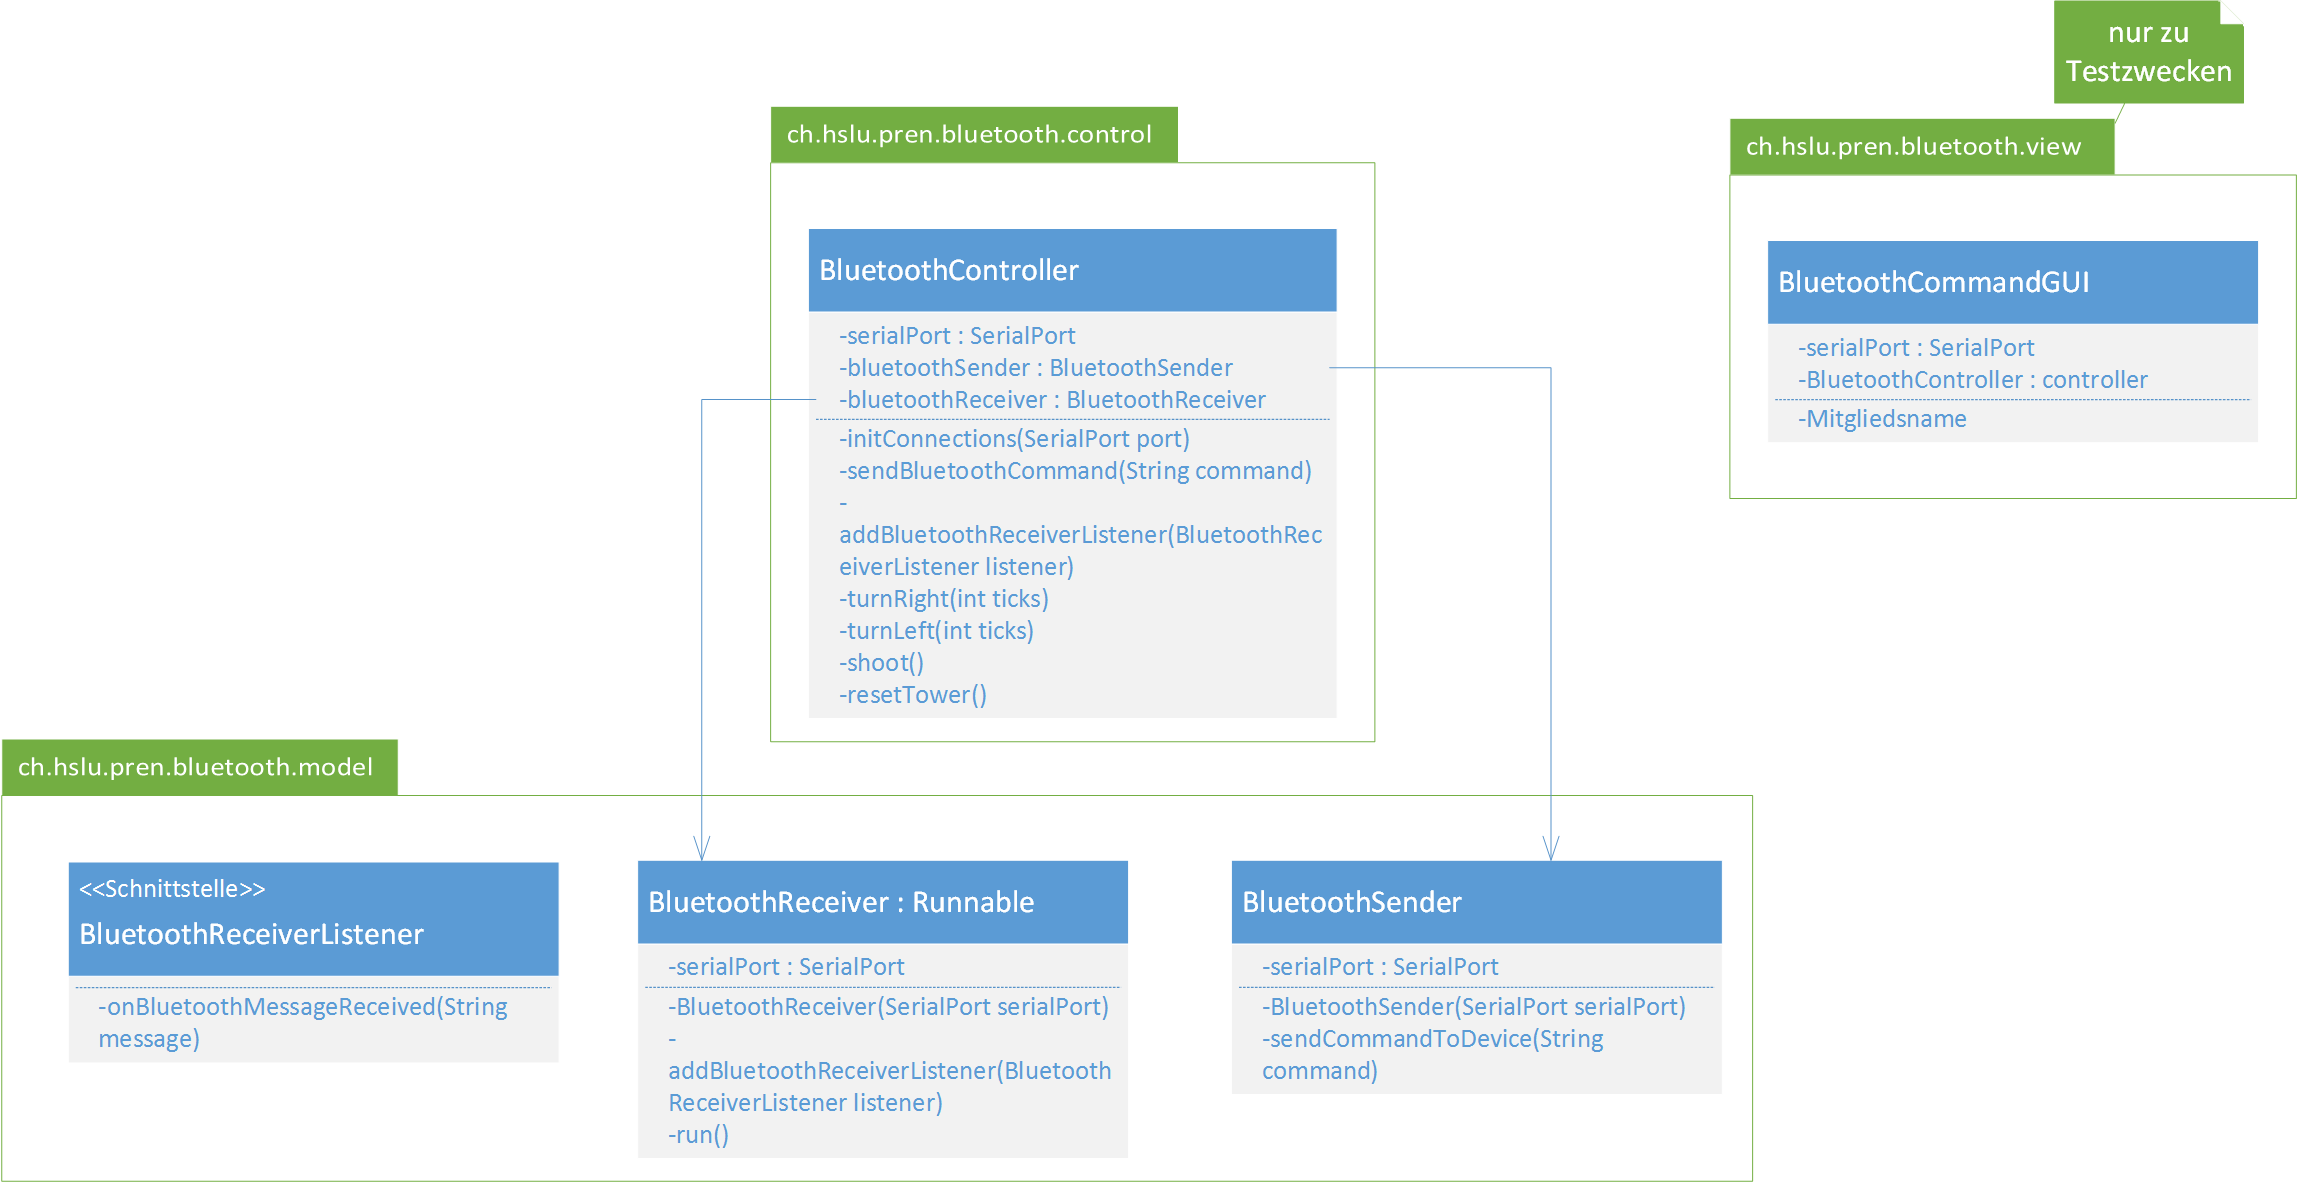
\includegraphics[width=1.0\textwidth]{../fig/Klassendiagramm_Bluetoothmodul.png}
        \end{column}
    \end{columns}
\end{frame}


\subsection{Kontrollplatine}
Als Steuerplatine kommt ein FRDM-KL25Z von Freescale zum Einsatz. 

\subsection{Ansteuerung Schrittmotor}
\label{sec:stepperdriver}
Die Ansteuerung für den Schrittmotor wird in der Gruppe PREN-ET entwickelt. 
(Siehe \ref{sec:pren-et} \nameref{sec:pren-et}) 
Daher werden hier nur Anpassungen für das Team 27 betrachtet. 
Die Platine mit der Schrittmotoransteuerung kann direkt auf das 
Controllerboard (siehe \ref{sec:control}) gesteckt werden.  Die weiteren 
Komponenten können mit einem Flachbandkabel an der Schrittmotoransteuerung 
angeschlossen werden. Das Bluetoothmodul wird direkt auf die 
Schrittmotorsteuerung gesteckt. 
\begin{figure}[h!]
    \centering
    \includegraphics[width=0.7\textwidth]{fig_pcb/DSC02908.JPG}
    \caption{Ansteuerung Schrittmotor}
    \label{fig:dc}
\end{figure}


\subsection{Fachgruppe Elektrotechnik}
\label{sec:pren-et}
Elektrotechnik-Studierende aus mehreren Gruppen haben sich
zusammengeschlossen, um gemeinsame Probleme anzugehen. Dabei handelt es sich
um die benötigte Hard- und Software, um Motoren anzusteuern
und gegebenenfalls zu regeln. In diesem Zusammenschluss werden drei Gruppen
gebildet, um Lösungen für DC-, Stepper- und Brushless-Motoren auszuarbeiten.
Die Idee besteht darin, dass nicht jede Gruppe für dasselbe Problem womöglich 
denselben Lösungsansatz verfolgt, sondern die Ressourcen kombiniert,
Synergien nutzt, um eine bessere Lösung zu erarbeiten. Auf diese Weise kann
das teamübergreifende Arbeiten im Rahmen des PREN erlernt und
geübt werden. Somit wird Idee der Interdisziplinarität im erweiterten Sinn
Rechnung getragen. Die Gruppen und deren Mitglieder sind in 
\autoref{tab:pren-et-members} aufgeführt.
\begin{table}[h!]
    \centering
    \begin{zebratabular}{lllccc}
        \rowcolor{gray} 
        Team & Mitglied         & Github    & DC          & BLDC        & Stepper     \\
        27   & Daniel Winz      & daniw     &             & \textbullet & \textbullet \\
        32   & Yves Studer      & ystuder   &             & \textbullet &             \\
        33   & Flavio Kreiliger & Flavinsky & \textbullet &             & \textbullet \\
        38   & Bettina Wyss     & BettyET   &             &             & \textbullet \\
        39   & Ervin Mazlagi\'c & ninux     & \textbullet &             &             \\
    \end{zebratabular}
    \caption{Übersicht der PREN-ET Projektgruppen}
    \label{tab:pren-et-members}
\end{table}
Für den Austausch und die Ablage von Daten und Unterlagen wird die Plattform 
Github ausgewählt, da damit via Git\footnote{Verteiltes 
Versionskontrollsystem} versioniert werden kann. Dazu wird auf Github die 
Organisation PREN-ET gegründet. Diese ist unter 
\url{https://github.com/PREN-ET} einsehbar. für die einzelnen Projekte werden 
Repositories angelegt. Diese sind in \autoref{tab:pren-et-repos} aufgeführt. 
\begin{table}[h!]
    \centering
    \begin{zebratabular}{p{0.09\textwidth}p{0.37\textwidth}p{0.4\textwidth}}
        \rowcolor{gray} 
        Repository  & Link         & Beschreibung \\
        info        & \url{https://github.com/PREN-ET/info}    & Allgemeine Informationen zur Organisation von PREN-ET \\
        doc         & \url{https://github.com/PREN-ET/doc}     & Dokumentation \\
        dc          & \url{https://github.com/PREN-ET/dc}      & Treiber für Gleichstrommotoren \\
        bldc        & \url{https://github.com/PREN-ET/bldc}    & Treiber für Brushless Motoren \\
        stepper     & \url{https://github.com/PREN-ET/stepper} & Treiber für Schrittmotoren \\
        frdm        & \url{https://github.com/PREN-ET/frdm}    & Beispiele zur Ansteuerung mittels FRDM-KL25Z \\
    \end{zebratabular}
    \caption{Übersicht der PREN-ET Repositories}
    \label{tab:pren-et-repos}
\end{table}

\subsection{Turm}
Der Turm dient als Verbindungselement des Balllager und des grösseren 
Zahnrades der Drehvorrichtung. Ausgeführt wurde die gesamte Konstruktion aus 
Aluminiumblech. Der Platz im Inneren wird zum Verstauen der 
Elektronikkomponenten verwendet.

\subsection{Ballbeförderung}
\begin{frame}
    \frametitle{Balllager}
    \begin{columns}
        \begin{column}{0.7\textwidth}
            \centering
            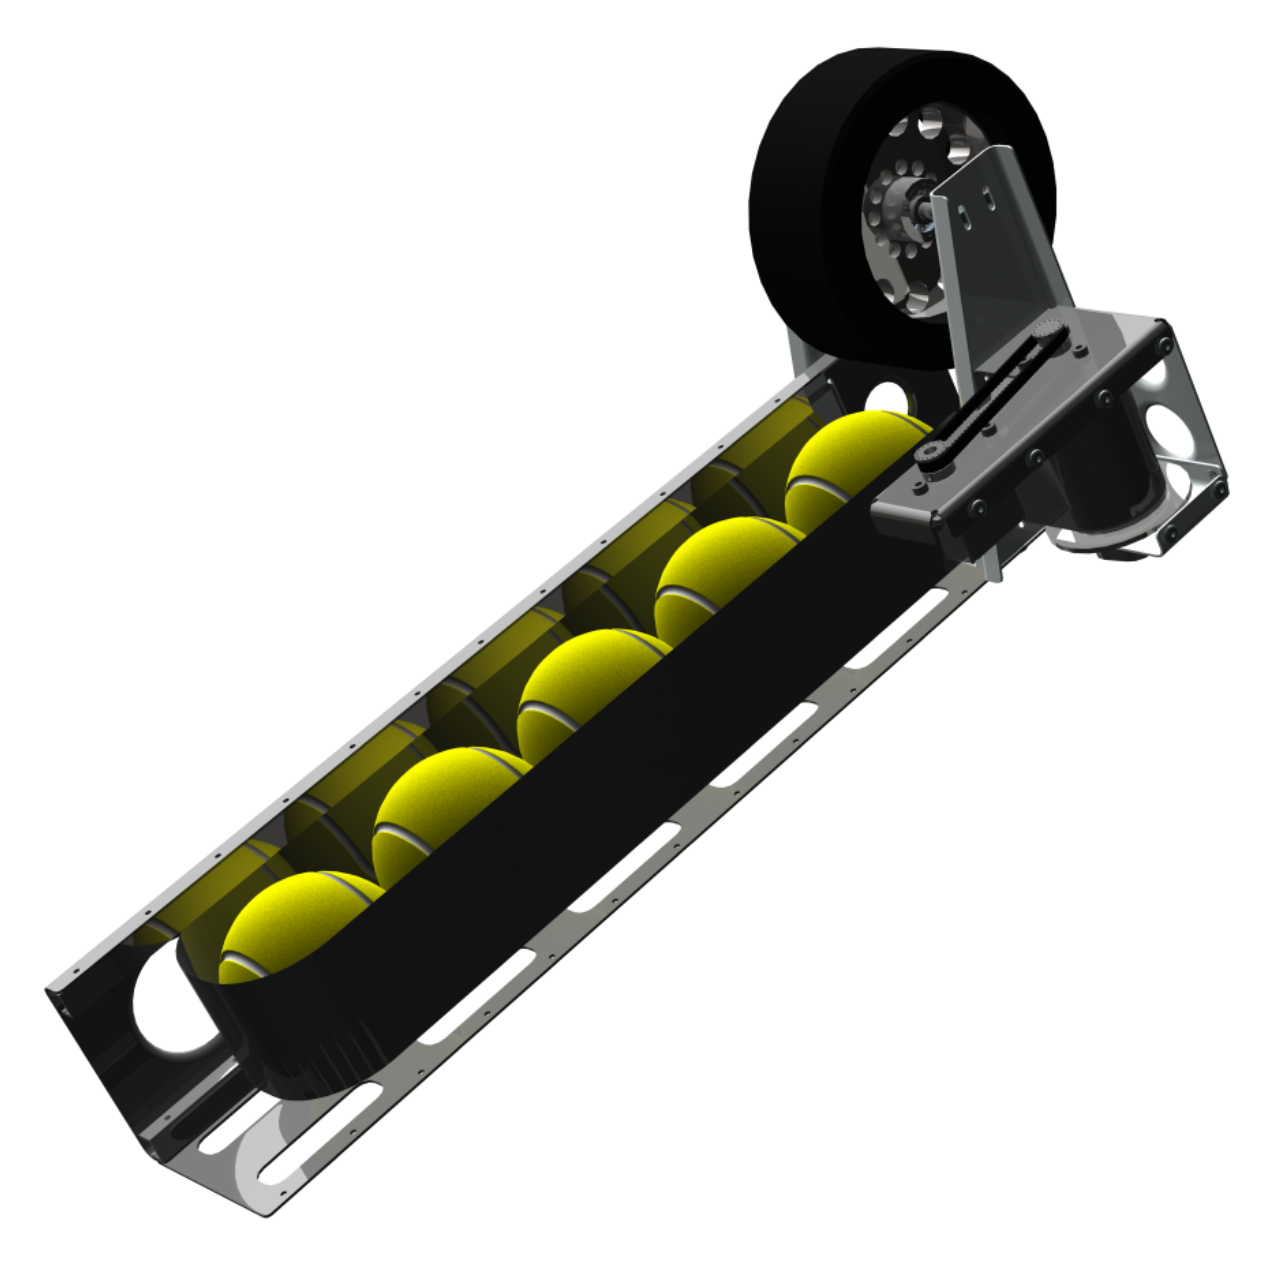
\includegraphics[width=1.0\textwidth]{FotosM/Bild7.png}
        \end{column}
    \end{columns}
\end{frame}
\begin{frame}
    \frametitle{Ballnachschub}
    \begin{columns}
        \begin{column}{0.8\textwidth}
            \centering
            \includegraphics[width=1.0\textwidth]{../doc/fig/DSC02958.JPG}
        \end{column}
    \end{columns}
\end{frame}
\begin{frame}
    \frametitle{Ballbeförderung}
    \begin{columns}
        \begin{column}{0.8\textwidth}
            \centering
            \includegraphics[width=1.0\textwidth]{../doc/fig/DSC02958.JPG}
        \end{column}
    \end{columns}
\end{frame}

\subsection{Ansteuerung BLDC Motor}
Die Ansteuerung für den BLDC Motor\footnote{\textbf{B}rush\textbf{L}ess 
\textbf{D}irect \textbf{C}urrent Motor} wird in in der Gruppe PREN-ET 
entwickelt. (Siehe \ref{sec:pren-et} \nameref{sec:pren-et})

\subsection{Ansteuerung Motor Ballnachschub}
\label{sec:dc}
Die Ansteuerung für den Motor für den Ballnachschub wird in in der Gruppe 
PREN-ET entwickelt. (Siehe \ref{sec:pren-et} \nameref{sec:pren-et})
Daher werden hier nur Anpassungen für das Team 27 betrachtet. 
\begin{figure}[h!]
    \centering
    \includegraphics[width=0.7\textwidth]{fig_pcb/DSC02909.JPG}
    \caption{Ansteuerung Ballnachschub}
    \label{fig:dc}
\end{figure}

\subsection{Energieversorgung}
Der Schrittmotor und der BLDC Motor werden mit einer Spannung von 48\si{\volt} 
betrieben. Der DC Motor für die Ballnachführung und die Kontrollplatine werden 
mit einer Spannung von 5\si{\volt} versorgt. Dazu werden Netzteile aus Servern 
verwendet. Davon werden vier in Serie geschaltet um die notwendige Spannung 
von 48\si{\volt} zu erreichen. Um Kurzschlüsse zu vermeiden, müssen die 
Netzteile potentialfrei gemacht werden. Bei den verwendeten Netzteilen vom Typ 
PS-3701-1 von HP wird die Sekundärseite mit einer Schraube elektrisch mit dem 
Gehäuse verbunden. Das Gehäuse ist mit PE verbunden und somit geerdet. Diese 
Schraube wird durch eine Kunststoffschraube ersetzt. Ausserdem ist der Abstand 
vom Gehäuse zur Platine an der Austrittsstelle der Platine sehr klein und kann 
zu unerwünschten Kurzschlüssen führen. Daher wird mit einem isolierenden 
Streifen aus FR4 einem allfälligen Kurzschluss vorgebeugt. 

\begin{frame}
    \frametitle{Ablauf}
    \begin{columns}
        \begin{column}{1\textwidth}
            \centering
            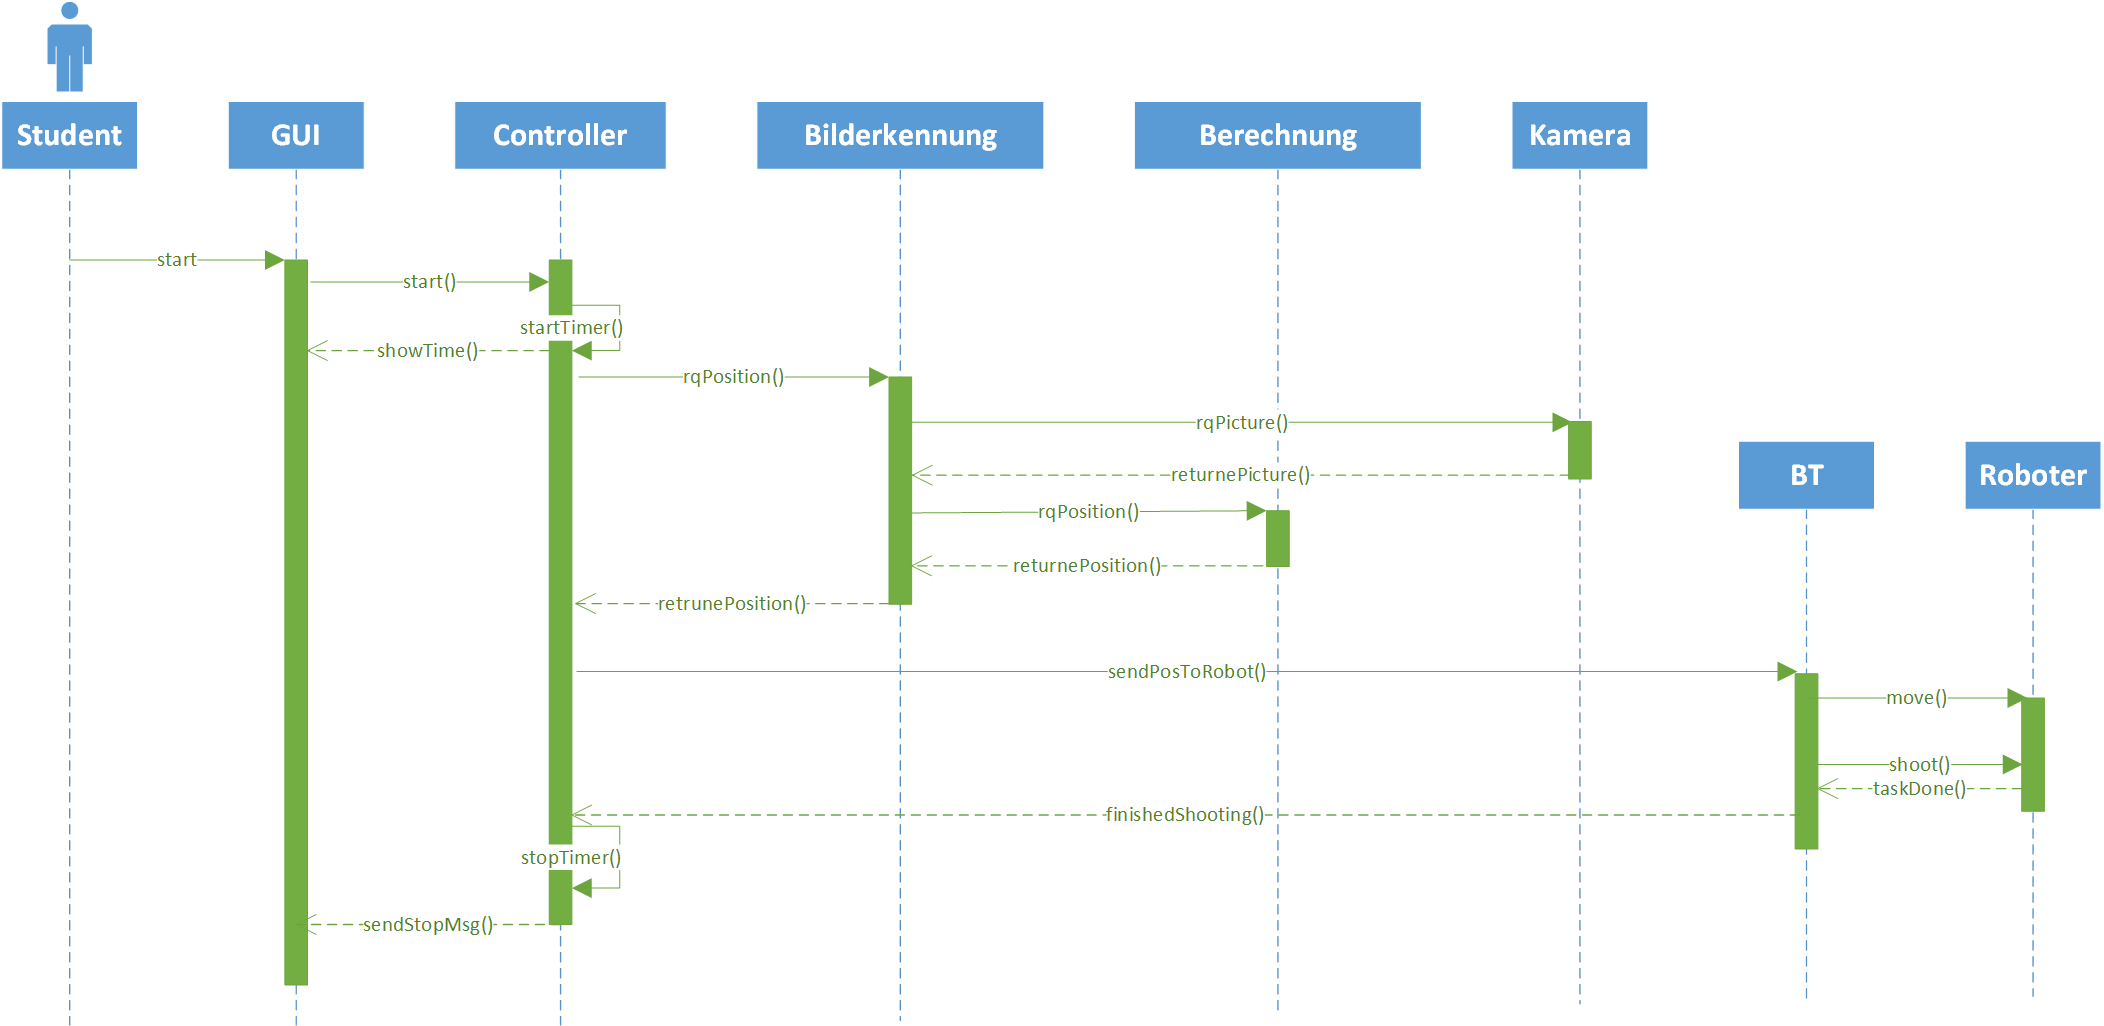
\includegraphics[width=1.0\textwidth]{../doc/fig/Sequenzdiagramm.png}
        \end{column}
    \end{columns}
\end{frame}


\section{Kenndaten}
\begin{frame}
    \begin{columns}
        \begin{column}{0.50\textwidth}
            \centering
            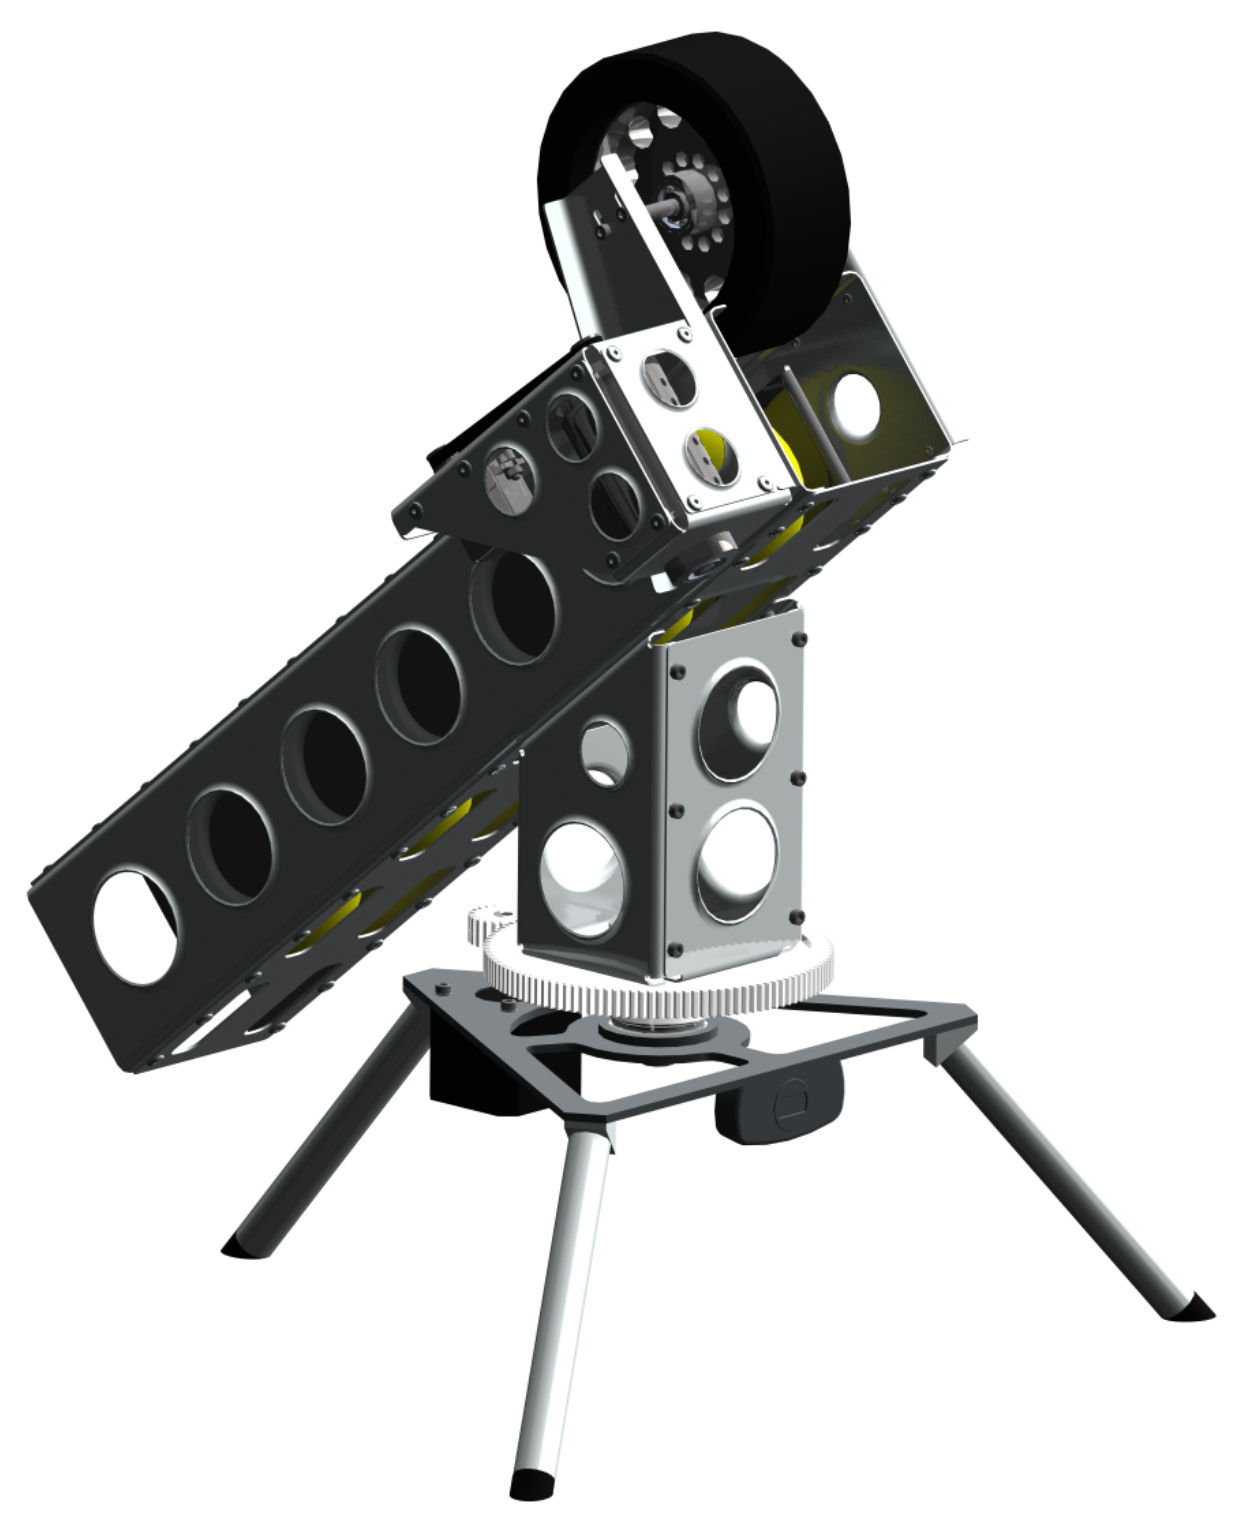
\includegraphics[width=1.00\textwidth]{../doc/fig/Bild_mit_Kamera.png}
        \end{column}
        \begin{column}{0.50\textwidth}
            \begin{block}{Kenndaten Twentyseven}
                \begin{itemize}
                    \item Gewicht 1932\si{\gram}
                    \item Zeit: 3\si{\second}
                    \item Treffsicherheit: 5/5
                \end{itemize}
            \end{block}
        \end{column}
    \end{columns}
\end{frame}

\section{Rückblick - Ausblick} % Peter
\begin{frame}
	\begin{block}{So wars - So wirds}
		\begin{itemize}
			\item Team
			\begin{itemize}
                \item
				%\item Harmonie
				%\item Nicht immer ganz ernst
				%\item Zielorientiert
			\end{itemize}
			\item Aufgabe
			\begin{itemize}
                \item
				%\item Aufteilung
				%\item Umfang
				%\item Empfinden
			\end{itemize}
			\item Wettbewerb
			\begin{itemize}
                \item
				%\item Endlich loslegen 
				%\item Optimistisch
			\end{itemize}
		\end{itemize}
	\end{block}
\end{frame}

